\documentclass[11pt]{article}
\usepackage[margin=1in]{geometry}
\usepackage[T1]{fontenc}
\usepackage{lmodern}
\usepackage{amsmath,amssymb,amsthm,mathtools,mathrsfs}
\usepackage{microtype,booktabs,enumitem,graphicx}
\usepackage{tikz}
\usetikzlibrary{arrows.meta,positioning,calc}
\usepackage[hidelinks]{hyperref}
\hypersetup{pdftitle={Bloch's Law for Finite-Range Heisenberg Ferromagnets in Three Dimensions},pdfauthor={OpenAI},pdfsubject={Low-temperature asymptotics of spontaneous magnetization}}
\numberwithin{equation}{section}
\allowdisplaybreaks[2]
\setlength{\emergencystretch}{2em}
\setcounter{tocdepth}{1}
\newtheorem{theorem}{Theorem}[section]
\newtheorem{proposition}[theorem]{Proposition}
\newtheorem{lemma}[theorem]{Lemma}
\newtheorem{corollary}[theorem]{Corollary}
\theoremstyle{definition}
\newtheorem{definition}[theorem]{Definition}
\theoremstyle{remark}
\newtheorem{remark}[theorem]{Remark}
\newcommand{\Q}{\mathbb Q}
\newcommand{\R}{\mathbb R}
\newcommand{\C}{\mathbb C}
\newcommand{\Z}{\mathbb Z}
\newcommand{\N}{\mathbb N}
\newcommand{\ind}[1]{\mathbf1_{#1}}
\DeclarePairedDelimiter{\norm}{\lVert}{\rVert}
\DeclareMathOperator{\Tr}{Tr}
\DeclareMathOperator{\diag}{diag}
\DeclareMathOperator{\dist}{dist}
\DeclareMathOperator{\rad}{rad}
\DeclareMathOperator{\supp}{supp}
\DeclareMathOperator{\Div}{div}
\DeclareMathOperator{\sgn}{sgn}
\title{Bloch's Law for Finite-Range Heisenberg\\Ferromagnets in Three Dimensions}
\author{OpenAI}
\date{October 5, 2026}
\begin{document}
\maketitle
\begin{abstract}
We prove Bloch's $T^{3/2}$ law for the spontaneous magnetization of
three-dimensional quantum Heisenberg ferromagnets at every fixed positive
quantum spin. The result holds for every nonnegative symmetric finite-range
interaction whose support generates $\Z^3$, including spatially anisotropic
couplings. The leading magnetization deficit has the exact coefficient
determined by the determinant of the quadratic one-magnon dispersion.
The thermodynamic limit is taken before the right field derivative at zero,
and the low-temperature limit is taken last.
\end{abstract}
\tableofcontents
\section{Introduction}
\label{sec:introduction}

Bloch's law predicts that the spontaneous magnetization of a
three-dimensional ferromagnet falls below its fully polarized value by
an amount proportional to $T^{3/2}$ at low temperature. We prove this
law for the quantum Heisenberg ferromagnet at every fixed spin, allowing
any nonnegative symmetric finite-range interaction whose support
generates the lattice. The interaction may be spatially anisotropic and need not
contain the ordinary nearest-neighbor bonds. Its quadratic dispersion
determines the leading coefficient.

\subsection{The model and the result}

Fix $S\in\{\tfrac12,1,\tfrac32,\ldots\}$. The spin space at each
site is $\mathfrak h_S=\C^{2S+1}$, with orthonormal basis
$(e_m)_{m=-S}^S$ and operators
\[
 S^ze_m=me_m,\qquad
 S^+e_m=\sqrt{S(S+1)-m(m+1)}\,e_{m+1}\quad(m<S),\qquad S^+e_S=0.
\]
Set $S^-=(S^+)^*$, $S^x=(S^++S^-)/2$, and
$S^y=(S^+-S^-)/(2i)$. A subscript specifies the site where an operator
acts. Let $J:\Z^3\to[0,\infty)$ have finite support and satisfy
\begin{equation}
 J(0)=0,\qquad J(z)=J(-z),\qquad
 \langle z:J(z)>0\rangle_{\Z}=\Z^3.
 \label{eq:interaction}
\end{equation}
On $\Lambda_N=[-N,N]^3\cap\Z^3$, with free boundary, define
\begin{equation}
 H^J_{S,N}=-\frac12\sum_{x,y\in\Lambda_N}
               J(y-x)\boldsymbol S_x\cdot\boldsymbol S_y,
 \qquad M_{S,N}=\sum_{x\in\Lambda_N}S_x^z.
 \label{eq:hamiltonian}
\end{equation}
The sum counts each unordered bond twice; the factor $1/2$ removes
that duplication. We set the lattice spacing, Boltzmann constant, and
$\hbar$ equal to one, so $T=\beta^{-1}$.

For $\beta>0$ and $h\in\R$, put
\begin{equation}
 p_\beta(h)=\lim_{N\to\infty}\frac1{\beta|\Lambda_N|}
       \log\Tr e^{-\beta(H^J_{S,N}-hM_{S,N})},
 \qquad m_{S,J}(\beta)=\partial_h^+p_\beta(0).
 \label{eq:pressure-magnetization}
\end{equation}
The finite-range pressure limit exists and is convex and $S$-Lipschitz;
Section~\ref{sec:pressure} recalls the proof. Rotation by $\pi$ about
the $x$-axis makes the pressure even, so $m_{S,J}(\beta)\in[0,S]$.
The derivative selects the magnetization in a field tending to zero
through positive values after the thermodynamic limit.

Define the positive definite matrix
\begin{equation}
 D_{S,J}=\frac S2\sum_{z\in\Z^3}J(z)zz^{\mathsf T}.
 \label{eq:diffusion-matrix}
\end{equation}
It is the quadratic coefficient of the one-magnon dispersion:
\begin{equation}
 \varepsilon_{S,J}(k)=S\sum_zJ(z)(1-\cos(k\cdot z))
       =k^{\mathsf T}D_{S,J}k+O(|k|^4).
 \label{eq:dispersion}
\end{equation}
Positive definiteness follows because the interaction support spans
$\R^3$.

\begin{theorem}[Bloch's law]
\label{thm:main}
For every fixed $S\in\{\tfrac12,1,\tfrac32,\ldots\}$ and every
interaction satisfying \eqref{eq:interaction},
\begin{equation}
 \lim_{\beta\to\infty}\beta^{3/2}\bigl(S-m_{S,J}(\beta)\bigr)
   =\frac{\zeta(3/2)}{8\pi^{3/2}\sqrt{\det D_{S,J}}}.
 \label{eq:bloch-law}
\end{equation}
\end{theorem}

For $J(\pm e_j)=1$ and all other couplings zero, $D_{S,J}=SI$;
the theorem gives the usual nearest-neighbor coefficient
$\zeta(3/2)/(8\pi^{3/2}S^{3/2})$. The order of limits is part of
the assertion: first volume tends to infinity at fixed $\beta,h$,
then $h\downarrow0$, and finally $\beta\to\infty$, with $S,J$ fixed.

\subsection{Historical context and dependencies}

Bloch derived the $T^{3/2}$ reduction from long-wavelength spin waves
\cite{Bloch1930}. The bosonic representation of Holstein and Primakoff
\cite{HolsteinPrimakoff1940} and Dyson's analysis of spin-wave interactions
\cite{Dyson1956a,Dyson1956b} developed the low-temperature expansion.
In particular, Dyson identified the interaction contribution to the
magnetization at order $T^4$; his estimates of the remaining higher-order
terms were not a rigorous fixed-spin proof of the asymptotic law
\cite[Section~9]{Dyson1956b}. The leading coefficient in
\eqref{eq:bloch-law} is obtained from the low-temperature density of ideal magnons with quadratic
energy $k^{\mathsf T}D_{S,J}k$. The issue is to justify this coefficient
for the interacting spin system and the field derivative in
\eqref{eq:pressure-magnetization}.

Rigorous ordering theory distinguishes sharply between dimensions and
between classical and quantum models. Mermin and Wagner excluded
positive-temperature spontaneous magnetic order for the one- and
two-dimensional isotropic Heisenberg models under their finite-range
hypotheses \cite{MerminWagner1966}. Infrared bounds proved symmetry
breaking for classical models \cite{FSS1976}, and Dyson, Lieb, and Simon
established ordering for classes of quantum antiferromagnets
\cite{DLS1978}. These developments left the standard three-dimensional
quantum ferromagnet as a separate problem, recorded by Lieb
\cite{Lieb1999} and still discussed as open in recent accounts
\cite{Seiringer2025,BjornbergRyan2026}. The distinct companion manuscript
\cite[Theorem~1.1]{Ordering} proves low-temperature magnetized equilibrium states
for the nearest-neighbor quantum ferromagnet. We use its finite-set
algebra and deterministic lattice geometry, with their precise
hypotheses stated at the points of use.

The free energy has a different rigorous history. Conlon and Solovej
\cite{ConlonSolovej1991} and T\'oth \cite{Toth1993} obtained bounds for
spin $1/2$. Correggi, Giuliani, and Seiringer proved the leading
low-temperature free-energy asymptotic for the nearest-neighbor model
on $\Z^3$ at every fixed spin \cite[Theorem~2.1]{CGS2015}. A zero-field free-energy estimate
does not by itself control the one-sided field derivative that defines
spontaneous magnetization. Our proof therefore estimates the observable
through a representation that remains uniform under arbitrary extra
up-spin constraints, and only then passes to pressure increments.

The probabilistic representation belongs to the random-interchange
approach of T\'oth \cite{Toth1993}; the symmetric-slot realization of
higher spin is described by Nachtergaele \cite{Nachtergaele1994}.
The pin argument uses the stable-polynomial approach to negative
dependence developed by Borcea, Br\"and\'en, and Liggett \cite{BBL2009}. Diffusive smoothing uses the
energy method of Nash \cite{Nash1958}. The companion \cite{Ordering}
provides the particular stable exchange symbols, presence inequality,
local lattice inequality, and routed unit flows used below. We prove
here the finite-range pin bootstrap, the quantitative long-return
bound, and the comparison that recovers the full dispersion.

\subsection{How returns determine the coefficient}

Represent each spin by $\ell=2S$ spin-$1/2$ \emph{slots}. Independent
Poisson exchanges between slots, followed by a uniform permutation of
the slots at each site, form directed cycles over a time period of
length $\beta$. A cycle has a single up or down color. Constraining
all cycles through the boundary and through specified slot-time points
to be up defines a \emph{pin law}. If $E$ is its pin set and $i$ is
an unpinned slot-time point, a change of weights gives
\[
 d_E(i)=\frac{r(E,\{i\})}{1+r(E,\{i\})},
\]
where $d_E(i)$ is its down probability. Under the law with $i$ also
pinned, $r(E,\{i\})$ is the probability that the directed line from
$i$ returns to $i$ at positive elapsed time before meeting $E$.
Section~\ref{sec:pins} makes this identity precise and represents
$r$ by a walk on the slots left after exposing the cycles missing the
augmented pin set. The exposed environment repeats over periods, while
the walk uses fresh transition randomness on every traversal.

There are two geometric tasks. For rough estimates, choose three
linearly independent interaction vectors. They generate a sublattice
of finite index; on each of its cosets, the chosen bonds form a copy
of the ordinary cubic lattice. Section~\ref{sec:geometry} transfers
local Nash and flow estimates to these copies and compares their
energies with the full interaction energy. Section~\ref{sec:bootstrap}
then proves a sparse-pin estimate by downward induction on the pin
set. This induction supplies enough regular time for diffusion without
assuming a finite-range ordering theorem.

Sharp asymptotics require all interaction bonds. The ideal walk has
site jump rates $SJ(z)$, and its heat kernel $p_t^{S,J}$ satisfies
\[
 p_t^{S,J}(x,x)\sim\kappa t^{-3/2},\qquad
 \kappa=(4\pi)^{-3/2}(\det D_{S,J})^{-1/2}.
\]
After a full traversal the slot index is uniform, so the ideal
$n$-period return probability to a specified slot is
$\ell^{-1}p_{n\beta}^{S,J}(x,x)$. Summing over the $\ell$ slots at a
site cancels this factor, leaving the finite sums
$\kappa\sum_{n\le K}n^{-3/2}$ that approach the Bloch coefficient.
The selected sublattice is used only for estimates; the full jump
kernel determines this coefficient.

The main analytic difficulty is controlling arbitrarily late returns
in the same repeated environment. Section~\ref{sec:returns} truncates
a quadratic hitting-probability identity after $K$ periods. A mass
already spread for time comparable to $K\beta$ has a flow to infinity
with energy at most $C(K\beta)^{-1/2}$. Averaging over one further
period gives a remainder bounded by
$CK^{-1/2}\beta^{-3/2}+o_K(\beta^{-3/2})$, with $C$ independent of
$K$. Its $K=1$ case first improves the exposed-slot density to
$O(\beta^{-3/2})$.

This improved density permits the comparison in
Section~\ref{sec:ideal}. The ideal path rarely encounters an exposed
strand over a fixed number of periods. Splitting a return at its
midpoint combines that small encounter probability with diffusive
smoothing, giving an error $o_K(\beta^{-3/2})$ in each return entry.
The comparison retains the same exposed environment in both halves;
independence of their environments is unnecessary. The finite-return
comparison and the long-return remainder give matching upper and
lower down-probability bounds, with the lower bound requiring a
pin-free neighborhood of the starting point.

Finally, Section~\ref{sec:pressure} expresses a positive field as a
mixture of extra pins. The probability of selecting any given slot
is at most $1-e^{-\beta h}$, so the required neighborhood is free of
extra pins with probability tending to one as $h\downarrow0$ at fixed
$\beta,K$. Integrating the finite-volume derivative bounds before
taking the thermodynamic limit proves \eqref{eq:bloch-law} in the
stated order. The uniform pin estimates, the finite-index geometric
reduction, and the energy bound for a spread source are the reusable
parts of the argument.

\section{Exchange pictures and pinned returns}\label{sec:pins}

We express the magnetization through colored exchange cycles, then turn
pinning probabilities into one-particle return probabilities.  Two changes
of law are involved.  Pinning removes the color factor from cycles that
meet the pins.  Exposing the cycles that avoid the pins leaves a conditional
exchange process on the remaining slots.  The last part of this section
identifies its first return moment with an unconditioned Markov walk in the
exposed environment.  These constructions are finite-dimensional; the
spatial estimates begin in Section~\ref{sec:geometry}.

\subsection{Spin slots and the exchange law}

Fix $\beta>0$ and a cube $\Lambda=\Lambda_N$.  Set $\ell=2S$ and
\[
 b_0=\max\{|z|_\infty:J(z)>0\},\qquad
 \partial\Lambda=\{x\in\Lambda:
       \dist_\infty(x,\mathbb Z^3\setminus\Lambda)\le b_0\},\qquad
 \Lambda^\circ=\Lambda\setminus\partial\Lambda.
\]
No interaction bond joins $\Lambda^\circ$ to the exterior of $\Lambda$.
The \emph{slots} are the elements of
$V_\Lambda=\Lambda\times\{1,\ldots,\ell\}$.  Above each unordered
bond $\{x,y\}\subset\Lambda$ with $J(y-x)>0$, include all $\ell^2$
unordered slot pairs.  Write $\mathcal E_\Lambda$ for the resulting
slot edges and set
\[
 J_e=J(y-x),\qquad c_e=\frac{J_e}{2}
       \quad(e\text{ above }\{x,y\}),\qquad
 w_\Lambda=\sum_{e\in\mathcal E_\Lambda}J_e.
\]

Under the \emph{base law} $\mathbb P_{\rm b}$, every slot edge $e$
carries an independent Poisson process of rate $c_e$ on $[0,\beta)$.
At a mark the two slot lines exchange.  At the end of the interval,
independent uniform permutations of the slots at each site join time
$\beta$ to time $0$.  We call these within-site permutations the
\emph{seam completions}.  A picture $\omega$ consists of its marks and
completions.  Following its lines through repeated copies of the same
picture gives directed cycles.  Their intersections with the time-zero
layer are the cycles of a permutation of $V_\Lambda$.

Time belongs to $\mathbb R/\beta\mathbb Z$.  At an exchange we use the
slot just after that exchange, and at time zero we use the slot just
after the seam completion.  Deterministic times almost surely avoid
Poisson marks.  If $a_C$ is the number of time-zero slots on a cycle
$C$, then $\sum_Ca_C=\ell|\Lambda|$.  A cycle coloring is a choice
$\sigma_C\in\{-1,1\}$ for each cycle; its magnetization is
\[
                 M(\sigma)=\frac12\sum_Ca_C\sigma_C.
\]

\begin{proposition}[Loop representation]\label{prop:loop-representation}
For every finite cube, every $\beta>0$, and every real $h$,
\begin{equation}\label{eq:loop-partition}
 Z_\Lambda(h):=\Tr e^{-\beta(H^J_{S,N}-hM_{S,N})}
   =e^{\beta w_\Lambda/4}\,
           \mathbb E_{\rm b}\sum_\sigma e^{\beta hM(\sigma)}.
\end{equation}
At zero field the Gibbs spectral law of total magnetization is obtained
by weighting each picture by $2^{\#\{\text{cycles}\}}$, coloring its
cycles independently and fairly, and evaluating $M(\sigma)$.  More
precisely, for every function $\Phi$ on the finite spectrum of
$M_{S,N}$,
\begin{equation}\label{eq:loop-spectral-law}
 \frac{\Tr\bigl(e^{-\beta H^J_{S,N}}\Phi(M_{S,N})\bigr)}{Z_\Lambda(0)}
   =\frac{\mathbb E_{\rm b}\sum_\sigma\Phi(M(\sigma))}
           {\mathbb E_{\rm b}2^{\#\{\text{cycles}\}}}.
\end{equation}
\end{proposition}

\begin{proof}
This is the exchange representation of T\'oth~\cite{Toth1993}, with
the higher-spin symmetric-slot construction of
Nachtergaele~\cite[Section~2.2]{Nachtergaele1994}; see also
\cite[Lemma~2.1]{Ordering}.  At one site let $\psi_k$ be the normalized
sum of the elementary spin-$\tfrac12$ tensors having $k$ up spins,
$0\le k\le\ell$.  The sum of the slot $z$-spins acts on $\psi_k$
by $k-\ell/2$, and the sum of the raising operators acts by
$\sqrt{(\ell-k)(k+1)}\,\psi_{k+1}$.  These are the spin-$S$ matrices
under $k=S+m$.  Thus the physical space is the range of
\[
 \mathcal S_\Lambda=\prod_{x\in\Lambda}\mathcal S_x,
 \qquad \mathcal S_x=\frac1{\ell!}
                  \sum_{\kappa\in\mathfrak S_\ell}\mathcal U_{\kappa,x},
\]
where $\mathcal U$ denotes tensor permutation on the slot space.

The spin-$\tfrac12$ identity
$\boldsymbol s_i\cdot\boldsymbol s_j
 =\frac12\mathcal U_{(ij)}-\frac14I$ gives the lifted Hamiltonian
\[
 \widehat H=-\frac12\sum_eJ_e\mathcal U_e
                      +\frac14w_\Lambda I,
 \qquad \widehat M=\sum_{i\in V_\Lambda}s_i^z.
\]
The full sum over all slot pairs above each bond commutes with every
within-site permutation, and hence with $\mathcal S_\Lambda$.
The Poisson product $\varphi$ of the exchanges satisfies
\[
 \mathbb E_{\rm b}\mathcal U_\varphi
   =\exp\left\{\beta\sum_ec_e(\mathcal U_e-I)\right\}
   =e^{-\beta w_\Lambda/4}e^{-\beta\widehat H}.
\]
For example, the first equality follows from the matrix evolution with
generator $\sum_ec_e(\mathcal U_e-I)$; no commutation of individual
transpositions is needed.  Averaging the seam completions inserts
$\mathcal S_\Lambda$.  Taking the trace after multiplication by
$e^{\beta h\widehat M}$ proves \eqref{eq:loop-partition}: in the
elementary up/down basis, a tensor permutation has a nonzero diagonal
entry exactly when the coloring is constant on each cycle.  The same
calculation with any function of $\widehat M$ proves the spectral-law
assertion.
\end{proof}

\subsection{Pins, boundary approximation, and mark counts}

A \emph{pin} is a specified slot-time point.  Define the continuous
boundary pin set
\[
       D_0=\partial\Lambda\times\{1,\ldots,\ell\}
                                   \times(\mathbb R/\beta\mathbb Z).
\]
An \emph{allowed} pin set is $D=D_0\cup F$ with $F$ finite and
deterministic.  We also use finite pin sets before taking the boundary
limit.  For either type of set, put
\[
 n_D(\omega)=\#\{C:C\cap D=\varnothing\},\qquad
 \mathcal B_D(\omega)=\bigcup_{C:\,C\cap D=\varnothing}C,
 \qquad \mathcal Z_D=\mathbb E_{\rm b}2^{n_D},
\]
and define
\begin{equation}\label{eq:pinned-law}
 \mathbb P_D(d\omega)=\mathcal Z_D^{-1}2^{n_D(\omega)}
                                        \mathbb P_{\rm b}(d\omega).
\end{equation}
The normalizer obeys $1\le\mathcal Z_D\le2^{|V_\Lambda|}$.
In the associated zero-field color law, cycles meeting $D$ are up and
the remaining cycles receive independent fair colors.  Denote by
$d_D(i)$ the probability that a slot-time point $i$ is down.  Then
\begin{equation}\label{eq:down-free-cycle}
                  2d_D(i)=\mathbb P_D(i\in\mathcal B_D).
\end{equation}

\begin{lemma}[Dense boundary cuts]\label{lem:dense-boundary}
Let $F$ be a finite deterministic pin set and let $\mathcal T_n$ be
increasing finite sets of times containing zero, with dense union.
Set
\[
 D_n=F\cup\bigl(\partial\Lambda\times\{1,\ldots,\ell\}
                                      \times\mathcal T_n\bigr),
 \qquad D=F\cup D_0.
\]
Almost surely, $n_{D_n}=n_D$ and $\mathcal B_{D_n}=\mathcal B_D$ for
all sufficiently large $n$.  Moreover $\mathbb P_{D_n}$ converges to
$\mathbb P_D$ in total variation.  If bounded observables $X_n$
converge almost surely to $X$, with a common deterministic bound,
then $\mathbb E_{D_n}X_n\to\mathbb E_DX$.
\end{lemma}

\begin{proof}
There are finitely many marks per period, their times are distinct,
and seam completions preserve sites.  Every visit to the boundary
therefore contains a time interval of positive length and is detected
by a cut from the dense union.  There are finitely many cycles, so one
finite cut set eventually detects every boundary-touching cycle.
The asserted eventual equalities follow.  Since
$1\le2^{n_{D_n}}\le2^{|V_\Lambda|}$, bounded convergence applies both
to the weights and their positive normalizers.  This gives convergence
of the densities in $L^1(\mathbb P_{\rm b})$, and also the assertion
about observables.  This argument is at fixed volume.
\end{proof}

Under a pin law the marks need not be independent.  The following
uniform estimate on lists of distinct marks will suffice for all path
counts.  Let $\omega_{\rm m}$ be the mark counting measure on
$X_\Lambda=\mathcal E_\Lambda\times[0,\beta)$, and write
\[
             \lambda_{\rm b}(\{e\}\times dt)=c_e\,dt.
\]

\begin{lemma}[Factorial domination]\label{lem:factorial}
For an allowed or finite pin set $D$, an integer $j\ge1$, and a
nonnegative measurable function $F$ on $X_\Lambda^j$,
\begin{equation}\label{eq:factorial-bound}
 \mathbb E_D\sum_{(u_1,\ldots,u_j)\in(\omega_{\rm m})^j_{\ne}}
                         F(u_1,\ldots,u_j)
 \le 2^j\int F\,d\lambda_{\rm b}^{\otimes j}.
\end{equation}
Here the sum is over ordered tuples of distinct marks.  The estimate
also holds with any prescribed time order or time restrictions.
\end{lemma}

\begin{proof}
Inserting a transposition cuts and rejoins two strands.  It joins two
cycles or splits one cycle into two, leaving the other cycles
unchanged, and preserves the union of the affected strands and their
pin incidences.  Joining cycles cannot increase $n_D$.  On splitting,
a cycle avoiding $D$ produces two such cycles, while a cycle meeting
$D$ has at least one descendant that still meets $D$.  Thus $n_D$
increases by at most one, and the weight increases by at most two.
This statement
applies outside the null set of coincident marks or deterministic pin
times, and also to continuous boundary pins.

The Poisson insertion identity, with the seam fixed, is
\begin{align*}
 &\mathbb E_{\rm b}\left[2^{n_D(\omega)}
     \sum_{(u_1,\ldots,u_j)\in(\omega_{\rm m})^j_{\ne}}F(u_1,\ldots,u_j)
                                                        \right]\\
 &\qquad=\int F(u_1,\ldots,u_j)\,
       \mathbb E_{\rm b}2^{n_D(\omega+\sum_{a=1}^j\delta_{u_a})}
                          \prod_{a=1}^j\lambda_{\rm b}(du_a).
\end{align*}
Indeed, in the Poisson series the $k$-mark term has
$k!/(k-j)!$ ordered choices for the distinguished marks.  Cancelling
that factor against $1/k!$ and summing the remaining marks proves the
identity.  Nonnegativity justifies it even for infinite integrals.
The insertion bound and division by $\mathcal Z_D$ prove
\eqref{eq:factorial-bound}.
\end{proof}

We shall freely use the weaker constant $4^j$ in
\eqref{eq:factorial-bound}.  If an independent fresh Poisson family is
sampled as well, a mixed
list obeys the product of these bounds: each actual mark contributes
$4\lambda_{\rm b}$ and each fresh mark contributes
$\lambda_{\rm b}$.  This follows by independence and the two factorial
measures.  It is an unconditional statement under $\mathbb P_D$,
which is the law used when counting paths below.

\subsection{Single and simultaneous pin tests}

Let $E$ be allowed or finite, and let $T$ be a nonempty set of
$m_T=|T|$ distinct slot points at one deterministic time $\theta$,
disjoint from $E$.  Set $P=E\cup T$.  Repeating a sampled picture,
let $\mathcal R_i(E,T)$ be the event that the line from $i\in T$
visits $T$ at strictly positive elapsed time before visiting $E$.
Define
\begin{equation}\label{eq:pin-return-fraction}
 r(E,T)=\frac1{m_T}\sum_{i\in T}
                    \mathbb P_P\bigl(\mathcal R_i(E,T)\bigr).
\end{equation}
Pinning $T$ changes the picture law in this definition.  The next
proposition compares the changed law with the probability that $T$
lies on cycles avoiding the original pins.

\begin{proposition}[Pin identities]\label{prop:pin-identities}
For $E,T$ as above,
\begin{equation}\label{eq:pin-identities}
 d_E(i)=\frac{r(E,\{i\})}{1+r(E,\{i\})}\quad(i\notin E),
 \qquad
 \mathbb P_E(T\subseteq\mathcal B_E)\le(2r(E,T))^{m_T}.
\end{equation}
\end{proposition}

\begin{proof}
For $T=\{i\}$, write $r=r(E,\{i\})$ and
$A=\{i\in\mathcal B_E\}$. A line returns
to $i$ before $E$ exactly on $A$, so $r(E,\{i\})=\mathbb P_P(A)$.
Moreover $2^{n_E}=2^{n_P}(1+\ind{A})$, giving
$\mathcal Z_E=\mathcal Z_P(1+r)$ and
$\mathbb P_E(A)=2r/(1+r)$.  Equation~\eqref{eq:down-free-cycle}
proves the singleton identity.
This calculation applies directly to finite and allowed pin sets.

For the simultaneous bound, we use three precise finite-set facts from
\cite[Lemmas~3.2, 3.4, and 3.6]{Ordering}.  A nonzero polynomial is
\emph{stable} if it has no zero when every variable has positive
imaginary part.  The facts are as follows.
\begin{enumerate}[label=(\roman*),leftmargin=*]
\item Variable identification preserves stability.  Partial derivatives,
real specialization, and coefficientwise limits of uniformly bounded
degree preserve stability up to the zero polynomial.  In particular,
after identifying two variables as $t$, taking the coefficient of $t$
preserves stability up to zero.
\item If a permutation $\pi$ of a finite set $V$ is a product of
independent Bernoulli transpositions and deterministic permutations,
then
\[
            \mathbb E\prod_{j\in V}(x_j+y_{\pi(j)})
\]
is stable.  This also holds for independent products of finite-time
Poisson exchanges with arbitrary nonnegative rates and uniform
permutations on specified subsets.
\item If a random subset $A$ of a finite set has a stable generating
polynomial $\mathbb E\prod_{j\in A}y_j$, then for every subset $B$,
\[
                     \Pr(B\subseteq A)\le\prod_{j\in B}\Pr(j\in A).
\]
\end{enumerate}
These facts belong to the stable-polynomial method for negative
dependence developed in~\cite{BBL2009}.  They concern arbitrary finite
sets, with no spatial hypothesis.  To check the continuous-time scope
in (ii), subdivide a
finite interval into small slices and replace each edge clock in each
slice by its independent indicator of at least one mark.  Apply these
Bernoulli transpositions in a fixed order.  The products agree with the
Poisson products whenever no slice has two marks in total; the
probability of disagreement tends to zero.  A uniform permutation is
likewise a distributional limit of complete-graph Poisson exchanges:
the unit-time transition matrix on its finite permutation group has
all entries positive and preserves the uniform law, so it contracts
total variation distance to that law.  Thus the rates $c_e=J_e/2$
meet exactly the hypotheses of (ii).

For this bound, first suppose that $E$ is finite.  Cut the time circle at zero and
at every pin time in $P$.  Let $V$ be the disjoint union of the slot
layers at these cuts, and let $\pi$ follow a line from one cut to the
next cyclic cut.  Include the seam completion in the interval ending
at zero.  The interval maps are independent and use disjoint sets
of input $x$ variables and output $y$ variables.  Their stable symbols
therefore multiply to give the stable polynomial
\[
                  F_V=\mathbb E_{\rm b}
                         \prod_{j\in V}(x_j+y_{\pi(j)}).
\]

Delete an unpinned point $q\in V\setminus P$ by setting
$x_q=y_q=t$ and taking the linear coefficient in $t$.  For a fixed
permutation with predecessor $i$ and successor $j$ at a nonfixed $q$,
the two affected factors are $(x_i+t)(t+y_j)$, whose linear
coefficient is $x_i+y_j$.  This splices $i\to q\to j$ to $i\to j$.
A fixed point instead contributes the factor $2t$ and hence the
factor two.  Deleting all nonpins gives
\begin{equation}\label{eq:spliced-symbol}
 F_P=\mathbb E_{\rm b}\left[
         2^{n_P}\prod_{j\in P}(x_j+y_{\sigma(j)})\right],
\end{equation}
where $\sigma$ is the permutation taking each pin to its next pin
on the same cycle.  Each cycle avoiding $P$ contributes exactly one
factor two, when its final vertex is deleted.  The closure facts
give stability; the positive coefficients exclude the zero polynomial.

Differentiate \eqref{eq:spliced-symbol} in every $x_j$ with
$j\in P\setminus T$, set every remaining $x$ variable to zero, and
divide by $\mathcal Z_P$.  The result is the stable generating
polynomial
\begin{equation}\label{eq:pin-output-polynomial}
 G_T(\boldsymbol y)=\mathbb E_P\prod_{i\in T}y_{\sigma(i)}.
\end{equation}
It is nonzero because $G_T(\boldsymbol1)=1$, and it represents the
subset $\sigma(T)$ because its indices are distinct.  Counting the
outputs lying in $T$ gives
\[
 m_Tr(E,T)=\mathbb E_P|T\cap\sigma(T)|
                =\sum_{j\in T}\mathbb P_P(j\in\sigma(T)).
\]
Fact (iii) and the arithmetic--geometric mean inequality now imply
\[
              \mathbb P_P(T\subseteq\sigma(T))\le r(E,T)^{m_T}.
\]
The event $T\subseteq\sigma(T)$ is equivalent to
$T\subseteq\mathcal B_E$.  Indeed $|\sigma(T)|=|T|$, so the first
event says $\sigma(T)=T$; iterating $\sigma$ then meets only pins
of $T$ on every cycle through $T$, and meets all the pins on each
such cycle.  The converse follows by the same cycle description.

Deleting $m_T$ pins frees at most $m_T$ cycles.  Thus, pointwise,
\[
 2^{n_P}\le2^{n_E}\le2^{m_T}2^{n_P},
                   \qquad \mathcal Z_E\ge\mathcal Z_P>0.
\]
For $A=\{T\subseteq\mathcal B_E\}$, this yields
\[
 \mathbb P_E(A)
   \le 2^{m_T}\frac{\mathcal Z_P}{\mathcal Z_E}\mathbb P_P(A)
   \le (2r(E,T))^{m_T}.
\]

For $E=F\cup D_0$, replace $D_0$ by the finite cuts of
Lemma~\ref{lem:dense-boundary}, obtaining $E_n$ and $P_n=E_n\cup T$.
The simultaneous-free event and the weights converge almost surely.
The return events converge as well: follow each line from $i\in T$
until its first positive visit to $T$.  This horizon is finite because
the line eventually returns to $i$ on its finite permutation cycle.
Every boundary visit before that horizon contains a positive-duration
interval and is eventually detected.  Thus
$\ind{\mathcal R_i(E_n,T)}\to\ind{\mathcal R_i(E,T)}$.
Lemma~\ref{lem:dense-boundary} now passes the finite-pin inequality
to the limit.
\end{proof}

\subsection{Exposing the cycles that miss the pins}

The simultaneous pin inequality reduces the avoidance event to an average
return under $\mathbb P_P$.  We next separate the obstacles to that
return from the remaining exchanges.  From now on $E$ is allowed,
$T$ and $P$ are as above, and the outer picture law is $\mathbb P_P$.
Label a line by its slot at time zero.  Expose all labels belonging
to cycles missing $P$, their trajectories during one period, and their
endpoint mappings, including their seam images.  Write $\mathbf a$
for this exposure and $\mathscr H$ for its generated sigma-field.
At time $t$, the \emph{holes} $H_t=H_t(\mathbf a)$ are the slots
not occupied by exposed labels.  Their total number is constant.
Every pin is a hole at its pin time; every boundary slot is a hole
at every time.

For fixed $\mathbf a$, define a law $\mathbb Q_{\mathbf a}$ on the
remaining picture by the following operations.  While the hole set
is fixed, put independent rate-$c_e$ Poisson exchanges on the edges
whose endpoints are holes.  When an exposed label moves from a slot
to a hole, move that hole in the opposite direction into the vacated
slot.  Such a \emph{forced transport} is a fixed bijection between
the hole layers before and after the exposed jump.  Exchanges of two
exposed labels do not affect holes.  At the seam, independently at
each site, complete the revealed mapping by a uniform bijection
between its remaining source and target slots.  Let $G_P$ be the
event that every cycle of this remaining picture meets $P$, and put
\[
                         g_P(\mathbf a)=\mathbb Q_{\mathbf a}(G_P).
\]

\begin{proposition}[Exposure disintegration]\label{prop:exposure}
Almost surely under $\mathbb P_P$, $g_P(\mathbf a)>0$ and the
conditional remaining-picture law given $\mathscr H$ is
$\mathbb Q_{\mathbf a}(\,\cdot\mid G_P)$.

More precisely, for a deterministic initial label set
$A\subseteq V_\Lambda$, let $\mu_A$ be the base distribution of
its trajectories and endpoint mappings.  Let $F_A$ be the event
that these paths avoid $P$ and their endpoint set is $A$.  On $F_A$,
let $c_A(\mathbf a)$ be the number of cycles of their endpoint
permutation.  For any bounded measurable $\Phi$ of the exposure
and remaining picture $\omega_{\rm h}$,
\begin{equation}\label{eq:exposure-disintegration}
 \mathbb E_P\Phi(\mathbf a,\omega_{\rm h})
 =\frac1{\mathcal Z_P}\sum_{A\subseteq V_\Lambda}
     \int_{F_A}2^{c_A(\mathbf a)}
        \mathbb E_{\mathbb Q_{\mathbf a}}
                 [\ind{G_P}\Phi(\mathbf a,\omega_{\rm h})]
                                            \,\mu_A(d\mathbf a).
\end{equation}
In particular, the exposure marginal on this branch is
\begin{equation}\label{eq:exposure-marginal}
 \mathcal Z_P^{-1}\ind{F_A}2^{c_A(\mathbf a)}g_P(\mathbf a)
                                                   \,\mu_A(d\mathbf a).
\end{equation}
The same assertions hold for finite deterministic $P$.
\end{proposition}

\begin{proof}
We give the rate-dependent construction underlying
\cite[Proposition~4.1]{Ordering}.  Fix $A$ before sampling the base
picture.  On every edge $e$ take two independent rate-$c_e$ clocks.
Accept a mark from the first family when at least one endpoint
contains an $A$-label just before the mark; accept one from the second
family when neither endpoint does.

This produces the base exchange process.  Indeed, if
$c_{\rm tot}=\sum_ec_e>0$, the superposed clock has rate
$2c_{\rm tot}$.  At each of its times, conditionally on the past,
the accepted-edge or rejection outcome has probability
$c_e/(2c_{\rm tot})$ for edge $e$ and probability $1/2$ for
rejection.  These probabilities do not depend on the past or the
superposed waiting times.  Iterated conditioning and Poisson splitting
give independent accepted edge clocks of rates $c_e$.  If
$c_{\rm tot}=0$, the statement is immediate.

The $A$-label histories use only first-family clocks.  Given their
positions just before the seam, revealing their images under each
uniform site permutation leaves a uniform bijection of the remaining
slots, independently from site to site.  The histories, including
these revealed images, therefore do not use the second clock family
or the residual completions.  Conditional on those histories, the
second clocks restricted to the now fixed hole intervals remain
independent Poisson clocks, while the cross jumps give exactly the
forced transports.  This proves the base conditional kernel
$\mathbb Q_{\mathbf a}$ on $F_A$.

On $F_A$, the labels in $A$ form whole cycles missing $P$.  Requiring
$G_P$ makes them precisely all such cycles.  Consequently each
complete picture contributes to exactly one term in
\[
                    2^{n_P}
        =\sum_{A\subseteq V_\Lambda}\ind{F_A}2^{c_A}\ind{G_P},
\]
where a summand is zero off $F_A$.  Apply the base conditional kernel
to this finite sum and divide by $\mathcal Z_P$ to obtain
\eqref{eq:exposure-disintegration}.  Integrating out the remainder
gives \eqref{eq:exposure-marginal}, which gives zero outer mass to
$g_P=0$.  Dividing by $g_P$ on its positive set proves the asserted
conditional law.  All history spaces here are finite-jump path spaces
on finite state spaces, with finite endpoint data; they are standard
Borel spaces and admit the conditional kernels used above.
\end{proof}

The factor $g_P$ in \eqref{eq:exposure-marginal} is part of the
exposure law throughout the proof.  In particular, averaging a function
of the holes will always mean averaging under the actual $\mathbb P_P$
marginal.  At a fixed exposure, however, the next algebraic calculation
uses the unconditioned law $\mathbb Q_{\mathbf a}$.

\subsection{Removing the cycle condition from a first moment}

We record the finite-dimensional argument from
\cite[Lemma~4.2 and Proposition~4.3]{Ordering}, including its proof
to specify precisely why fresh transitions appear.  Matrices use the
column-forward convention: a permutation matrix obeys
$\Pi e_i=e_{\pi(i)}$.  For a matrix $M$, $\bigwedge^kM$ denotes
its action on alternating $k$-tensors; its matrix entries are the
$k\times k$ minors of $M$, and $\bigwedge^0M=1$.

\begin{lemma}[Exterior moments]\label{lem:exterior-moments}
Suppose a random permutation matrix $\Pi$ on a finite set is a
distributional limit of products of independent Bernoulli
transpositions and deterministic permutations.  If $K=\mathbb E\Pi$,
then
\begin{equation}\label{eq:exterior-moments}
            \mathbb E\bigwedge\nolimits^k\Pi=\bigwedge\nolimits^kK
                        \qquad(0\le k\le|V|).
\end{equation}
For every fixed exposure and finite set of cuts, the layered
permutation obtained under $\mathbb Q_{\mathbf a}$ by following
holes to the next cyclic cut has this property.
\end{lemma}

\begin{proof}
For a transposition matrix $T_{ij}$,
\[
                 T_{ij}-I=-(e_i-e_j)(e_i-e_j)^*.
\]
Every minor of $I+u(T_{ij}-I)$ is affine in $u$, since a term using
two columns of the rank-one perturbation has determinant zero.
Thus
\[
 \bigwedge\nolimits^k\bigl((1-u)I+uT_{ij}\bigr)
   =(1-u)\bigwedge\nolimits^kI+u\bigwedge\nolimits^kT_{ij},
\]
which proves the identity for one Bernoulli transposition.
Multiplicativity of exterior powers and independence preserve it
under products.  Deterministic permutations satisfy it directly,
and continuity of the minors on the finite matrix space passes it
to distributional limits.

For the hole picture, subdivide each interval between prescribed
changes and use the Bernoulli approximation already described.
Forced transports are deterministic bijections.  The residual seam
completions are uniform bijections, each expressible as a fixed
bijection composed with a uniform permutation; the latter has the
complete-graph exchange approximation described above.  Identify
every cut layer with a fixed set of $|H_t|$ elements.  The interval
maps act independently on separate copies of this set; their direct
sum followed by the deterministic cyclic shift of the layers is
the layered permutation.  A transposition in one block is a
transposition on the full layered set.  This verifies the required
product representation, before imposing $G_P$.
\end{proof}

\begin{proposition}[Conditional next-pin kernel]\label{prop:next-pin-kernel}
Let $V=I\sqcup B$ be a finite set with $I\ne\varnothing$.  Suppose
a random permutation matrix $\Pi$ satisfies
\eqref{eq:exterior-moments}, and let $K=\mathbb E\Pi$.  Let $G_I$
be the event that every cycle meets $I$.  On $G_I$, let $\Sigma$
be the column-forward permutation matrix on $I$ giving the next
positive visit to $I$.
Then
\begin{equation}\label{eq:all-hit-determinant}
                         \Pr(G_I)=\det(I-K_{BB}).
\end{equation}
If this probability is positive, then $K_{BB}$ is transient and
\begin{equation}\label{eq:conditional-next-pin}
 \mathbb E[\Sigma\mid G_I]
       =K_{II}+K_{IB}(I-K_{BB})^{-1}K_{BI}.
\end{equation}
The right-hand side is the first positive $I$-hitting kernel of
the Markov chain with independent transitions according to $K$.
If $B$ is empty, the determinant is one and the correction is zero.
\end{proposition}

\begin{proof}
The principal-minor expansion and \eqref{eq:exterior-moments} give,
for every fixed matrix $D$,
\begin{equation}\label{eq:determinant-expectation}
 \mathbb E\det(I-D\Pi)
  =\sum_k(-1)^k\Tr\left[(\bigwedge\nolimits^kD)
                           \mathbb E\bigwedge\nolimits^k\Pi\right]
  =\det(I-DK).
\end{equation}
Choose $D=\operatorname{diag}(W,I_B)$ with an arbitrary complex
$I\times I$ matrix $W$.  If a cycle lies in $B$, its indicator
vector is fixed by $D\Pi$, so the determinant vanishes.  On $G_I$,
$\Pi_{BB}$ is nilpotent and its resolvent follows the successive
nonpins on a permutation cycle.  Block elimination therefore gives
\[
 \det(I-D\Pi)
 =\det\left(I-W[\Pi_{II}+
               \Pi_{IB}(I-\Pi_{BB})^{-1}\Pi_{BI}]\right)
 =\det(I-W\Sigma).
\]
Consequently
\begin{equation}\label{eq:next-pin-determinant}
 \mathbb E[\ind{G_I}\det(I-W\Sigma)]
     =\det\begin{pmatrix}
             I-WK_{II}&-WK_{IB}\\
             -K_{BI}&I-K_{BB}
           \end{pmatrix}.
\end{equation}
Setting $W=0$ proves \eqref{eq:all-hit-determinant} without any
invertibility assumption.  When its value is positive,
$I-K_{BB}$ is invertible; taking the Schur complement in
\eqref{eq:next-pin-determinant} and dividing by that determinant yields
\[
 \mathbb E[\det(I-W\Sigma)\mid G_I]=\det(I-WH),
 \qquad H=K_{II}+K_{IB}(I-K_{BB})^{-1}K_{BI}.
\]
Replace $W$ by $tW$ and compare linear coefficients.  The identity
$\det(I-tWA)=1-t\Tr(WA)+O(t^2)$ shows that
$\Tr(W\mathbb E[\Sigma\mid G_I])=\Tr(WH)$ for every $W$.
Matrix units recover every entry, proving
\eqref{eq:conditional-next-pin}.

Finally, $K$ is nonnegative and doubly stochastic.  Its restriction
$K_{BB}$ is substochastic.  If some state of $B$ could never reach
$I$, its reachable set would contain a closed class and force the
eigenvalue one for $K_{BB}$, contradicting invertibility.  Finiteness
then supplies an integer $a$ and $\varepsilon>0$ such that every
state exits $B$ within $a$ steps with probability at least
$\varepsilon$.  Hence $\|K_{BB}^{an}\|_{1\to1}\le(1-\varepsilon)^n$
and
\[
                       (I-K_{BB})^{-1}=\sum_{n\ge0}K_{BB}^n.
\]
The first term in $H$ is a direct hit of $I$, and
$K_{IB}K_{BB}^nK_{BI}$ records a first hit after $n+1$ intervening
states of $B$.  This proves the asserted Markov interpretation.
\end{proof}

\subsection{The fresh walk}

Fix an exposure with $g_P(\mathbf a)>0$.  Repeat its hole sets,
forced transports, and revealed seam restrictions periodically.
The \emph{fresh walk} follows the one-particle transitions of
$\mathbb Q_{\mathbf a}$: it jumps across each available slot edge
at rate $c_e$, follows the forced transports, and at a seam uses a
fresh uniform residual completion.  Its random choices on disjoint
traversal intervals, including later repetitions of the same physical
interval, are independent.  Finite jump rates and finitely many
prescribed changes per period make this a nonexplosive Markov walk.
For $i\in T$, let $\tau_T^+$ be its first visit to $T$ at strictly
positive elapsed time and $\tau_E$ its first visit to $E$; an absent
visit has time infinity.  Put
\begin{equation}\label{eq:fresh-q}
             q_i(\mathbf a)=\Pr^{\rm walk}_{\mathbf a,i}
                                         (\tau_T^+<\tau_E).
\end{equation}

\begin{proposition}[Fresh-walk identity]\label{prop:fresh-walk}
For almost every exposure under $\mathbb P_P$ and every $i\in T$,
\[
       \mathbb P_P(\mathcal R_i(E,T)\mid\mathscr H)=q_i(\mathbf a).
\]
In particular,
\begin{equation}\label{eq:fresh-return}
                m_Tr(E,T)=\mathbb E_P\sum_{i\in T}q_i(\mathbf a).
\end{equation}
\end{proposition}

\begin{proof}
First use finitely many pins and take cuts at all pin times and
zero.  The unconditioned layered hole permutation under
$\mathbb Q_{\mathbf a}$ satisfies
Lemma~\ref{lem:exterior-moments}.  Conditional on every cycle hitting
the pins, Proposition~\ref{prop:next-pin-kernel} identifies its
next-pin first moment with independent transitions of its mean matrix.
Those transitions are exactly the fresh walk observed at the cuts.
Together with Proposition~\ref{prop:exposure}, this proves the
finite-pin assertion.

For an allowed $E=F\cup D_0$, fix an exposure for which the
disintegration holds and $g_P>0$.  Approximate the boundary by
increasing dense finite cuts and write $E_n=F\cup D_{0,n}$,
$P_n=E_n\cup T$.  The cuts include zero and all times in $P_n$.
Under the fixed unconditioned law $\mathbb Q_{\mathbf a}$, let
$G_n$ mean that every remaining cycle meets $P_n$, and put
$g_n=\mathbb Q_{\mathbf a}(G_n)$.

Every boundary visit of the remaining picture has positive residence
time.  Its Poisson marks almost surely avoid the finitely many
prescribed changes; seam completions preserve sites; and exposed
histories avoid the boundary, so forced transports cannot cause an
instantaneous boundary excursion.  Consequently
\[
              \ind{G_n}\uparrow\ind{G_P},\qquad
                         g_n\uparrow g_P>0.
\]
For all sufficiently large $n$, Proposition~\ref{prop:next-pin-kernel}
is therefore applicable with the pin layer $I=P_n$.  If $A_n$ is
the event that the next $P_n$-pin after $i$ is in $T$, it gives
\begin{equation}\label{eq:finite-cut-fresh-return}
 \frac{\mathbb Q_{\mathbf a}(G_n\cap A_n)}{g_n}
       =\Pr^{\rm walk}_{\mathbf a,i}(\tau_T^+<\tau_{E_n}).
\end{equation}
No assertion about the possibly singular earlier $n$ is needed.

In a fixed remaining picture the first positive return from $i$ to
$T$ is finite.  Detecting all boundary visits before that return
shows that $\ind{A_n}$ decreases to
$\ind{\mathcal R_i(E,T)}$.  Bounded convergence on the left of
\eqref{eq:finite-cut-fresh-return}, including its positive limiting
denominator, gives the return probability under
$\mathbb Q_{\mathbf a}(\,\cdot\mid G_P)$.

On the right use one uncensored fresh trajectory for all $n$.
The events decrease; every one requires $\tau_T^+<\infty$.
Any boundary visit before this finite time is detected by a dense
cut, again because it has positive duration.  Their intersection
is therefore exactly $\{\tau_T^+<\tau_E\}$ up to a null set.
Continuity from above proves convergence to \eqref{eq:fresh-q}.
The disintegration identifies the two limits, and averaging under
the exposure marginal \eqref{eq:exposure-marginal} proves
\eqref{eq:fresh-return}.
\end{proof}

We have obtained a Markov return problem in a periodic environment
whose missing slots are the exposed cycles.  The environment retains
its full pinned-law distribution, while the walk resamples its
transitions on every traversal.  The next section develops the
deterministic heat-flow estimates needed to bound these returns.

\section{Kernels and the geometry of available slots}\label{sec:geometry}

The fresh walk moves through a graph whose available slots change with
physical time.  We need two deterministic ways to control it: a Nash
inequality converts dissipation into diffusion, and flows to infinity
bound the pairing of a source mass with a test function by its Dirichlet
energy.  The first source bound permits many sparse starting points;
the second becomes sharper when a single source has already diffused.
We obtain both bounds on a fixed collection of nearest-neighbor
sublattices contained in the interaction graph.  The walk itself always
uses all interaction bonds.

\subsection{Coset coordinates and the killed kernels}

Choose linearly independent vectors \(a_1,a_2,a_3\) with \(J(a_j)>0\),
and let \(A\) be the integer matrix with these columns.  Such a choice
exists because the support of \(J\) generates \(\Z^3\).
The sublattice \(A\Z^3\) has finite index \(|\det A|\).  Fix
representatives \((u_\gamma)_{\gamma\in\mathfrak C}\) of its cosets and
write, uniquely,
\begin{equation}\label{eq:coset-coordinates}
 x=u_\gamma+A\bar x,
 \qquad \gamma\in\mathfrak C,\quad \bar x\in\Z^3.
\end{equation}
For \(z\in\Z^3\) and \(R\ge0\), put
\[
 B_R(z)=\{w\in\Z^3:|w-z|_\infty\le R\},
 \qquad
 \mathfrak B_R(z)=\{x\in\Z^3:\bar x\in B_R(z)\}.
\]
Thus \(\mathfrak B_R(z)\) contains a copy of the same coordinate ball
in every coset.  Each coset contains all nearest-neighbor edges of its
\(\bar x\)-coordinate lattice, since these edges are the displacements
\(\pm a_j\).  There is also a fixed integer \(B_*\ge1\) such that
\begin{equation}\label{eq:bond-coordinate-range}
 J(y-x)>0\quad\Longrightarrow\quad
 |\bar y-\bar x|_\infty\le B_*.
\end{equation}
Indeed, \(\bar y-\bar x=A^{-1}(y-x+u_\gamma-u_{\gamma'})\), and the
right side has only finitely many possibilities.  Constants below may
depend on this choice of coordinates, \(S,J\), and fixed geometric
radii, but never on the volume, pins, or subsequent scales.

Fix an exposure \(\mathbf a\) from Section~\ref{sec:pins} and a cut
\(\theta\).  Let \(U\) be the one-period fresh-walk kernel from the
holes at this cut back to the same holes, killed whenever it visits
\(\partial\Lambda\), including at its starting point.  The kernel
has no killing at other pins.  We use column-forward matrices: \(Uv\)
is the output mass when the input mass is \(v\).  Define
\begin{equation}\label{eq:one-period}
 U_+=U,\qquad U_-=U^*,\qquad
 Q=\frac{U+U^*}{2},\qquad A_Q=I-Q.
\end{equation}
The ordered kernel $U$ need not be self-adjoint. Its quadratic form
on real vectors agrees with that of $Q$, so the symmetric part is the
operator needed for the return-energy estimate.
The adjoint traversal reverses the order of all factors.  Between
prescribed changes the heat factors are symmetric; transports reverse
by their inverse bijections, and the adjoint of a uniform seam completion
is a uniform inverse completion.  Killing projections accompany these
factors in both directions.

Every interval kernel is an average of partial permutation matrices:
sample the simultaneous trajectories of all holes and retain precisely
those trajectories that survive the killing.  Consequently it is
nonnegative, with every row and column sum at most one, and contracts
counting \(1\)-, \(2\)-, and supremum norms.  For example, if \(K\)
is such a kernel, Cauchy--Schwarz gives
\[
 \sum_i|(Kv)_i|^2
 \le\sum_i\Bigl(\sum_jK_{ij}\Bigr)
              \Bigl(\sum_jK_{ij}|v_j|^2\Bigr)
 \le\sum_j|v_j|^2.
\]
These properties hold for adjoints, products, and further spatial
killing.  In particular \(Q\) is self-adjoint and a contraction, so
\(A_Q\) is positive semidefinite.

A split of a traversal always uses matching hole layers.  At a prescribed
transport or seam we distinguish its two sides and assign the operation
to exactly one of the adjoining factors.  Thus a full forward traversal
from the post-seam cut at zero includes its seam at the end.  Reversing
a traversal reverses this same ordered list.  Time integrals ignore the
finitely many instantaneous operations.

At time \(t\), extend the holes by making all \(\ell\) slots outside
\(\Lambda\) available.  Let \(\mathcal H_t\) be the resulting infinite
available-slot graph, with all pairs of available slots above each
interaction bond joined.  For a finitely supported real function \(v\)
on this graph, define
\begin{equation}\label{eq:full-energy}
 \mathcal D_t(v)=
 \sum_{e=\{i,j\}\in E(\mathcal H_t)}c_e\bigl(v(i)-v(j)\bigr)^2,
 \qquad c_e=\tfrac12 J(x_j-x_i).
\end{equation}
Each unoriented edge is counted once.  A killed vector is extended by
zero on killed slots, including the boundary and the exterior.
On a smooth interval, in elapsed time \(u\) in either traversal direction,
\begin{equation}\label{eq:norm-dissipation}
 \frac{d}{du}\|v(u)\|_2^2=-2\mathcal D_{t(u)}(v(u)).
\end{equation}
To verify this, pair the symmetric jump generator with \(v\); each
edge contributes \(-2c_e(v(i)-v(j))^2\).  Edges to killed slots retain
their exit rates and give the same expression with the killed value
zero.  There is no bond from \(\Lambda^\circ\) directly to the exterior,
so the infinite extension creates no extra term.  The same identity
holds after additional killing outside a fixed spatial set.  Squared
norm cannot increase at any instantaneous factor.

\subsection{Regular anchors and local diffusion}

For a coset \(\gamma\), let \(\mathcal H_t^\gamma\) contain its
available slots and only the nearest-neighbor edges in bar coordinates.
Write
\[
 \mathcal D_t^\gamma(v)
   =\frac12\sum_{\{i,j\}\in E(\mathcal H_t^\gamma)}
                   (v(i)-v(j))^2,
 \qquad c_0=\min_{1\le j\le3}J(a_j)>0.
\]
The graphs for different cosets have disjoint vertex sets, and their
edges are a subset of the full interaction edges.  Therefore
\begin{equation}\label{eq:energy-comparison}
 \mathcal D_t(v)\ge c_0
       \sum_{\gamma\in\mathfrak C}\mathcal D_t^\gamma(v).
\end{equation}
This inequality is the only place where the geometric subgraphs replace
the full graph; in particular it changes constants, not the diffusion
matrix that will determine Bloch's coefficient.

Fix
\[
 \alpha=\frac1{100},\qquad \nu=\frac1{300},\qquad
 L\ge\max\{6,\ell|\mathfrak C|\}.
\]
\begin{definition}[Sparse collections]\label{def:sparse}
A finite collection of slot points with site coordinates \((x_i)\) is
\emph{sparse} if
\begin{equation}\label{eq:sparse-growth}
 \#\{i:\bar x_i\in B_h(z)\}\le L(1+h)^\alpha
 \qquad(z\in\Z^3,\ h\ge0).
\end{equation}
Repeated bar coordinates count with their multiplicities, including
points from different cosets.  The same definition applies to a list of
centers in \(\Z^3\).  Every subcollection remains sparse.
\end{definition}

In coset \(\gamma\), call a coordinate site \emph{blocked} if it has
no available slot; denote this finite set by \(\mathcal O_t^\gamma\).
Join blocked sites whose supremum distance is at most eight.
For \(w\in\mathcal O_t^\gamma\), let \(\mathcal C_t^\gamma(w)\)
be its component and put
\[
 \operatorname{rad}_w\mathcal C_t^\gamma(w)
   =\max_{v\in\mathcal C_t^\gamma(w)}|v-w|_\infty.
\]
Boundary sites and all sites outside \(\Lambda\) have every slot
available.  Partial exposure at a site is permitted: an unblocked site
can have any number of available slots between one and \(\ell\).

We recall the precise local-connectivity input from
\cite[Lemma~5.5]{Ordering}.  For every fixed integer \(b\ge1\), there
is an integer \(\rho(3,b)\ge b+1\) such that if
\(u,v\notin F\subset\Z^3\), \(|u-v|_\infty\le b\), and
\(\#(F\cap B_{\rho(3,b)}(u))<6\), then a nearest-neighbor path from
\(u\) to \(v\) avoids \(F\), stays in that ball, and has length at
most \((2\rho(3,b)+1)^3\).  Fix an integer, as in the radius choice of
\cite[Equation~(5.13)]{Ordering},
\begin{equation}\label{eq:geometric-radius}
 M_*\ge\max\{48,\rho(3,44)+2\}.
\end{equation}
The numbers 44 and 48 cover the bounded connections around components
of at most five blocked sites.  Fix a lower threshold \(R_0\) large
enough for all subsequent deterministic estimates; it includes
\(R_0\ge M_*+47\).  This threshold depends only on the fixed geometry.

\begin{definition}[Regular slice]\label{def:regular}
A slice \(t\) is \emph{regular for the anchor \(z\) at radius \(R\)}
if the following hold in every coset \(\gamma\):
\begin{enumerate}
 \item for every \(w\in B_{11R}(z)\),
 \(\#(\mathcal O_t^\gamma\cap B_{M_*}(w))<6\);
 \item for every \(w\in\mathcal O_t^\gamma\setminus B_{10R}(z)\),
 \(\operatorname{rad}_w\mathcal C_t^\gamma(w)
       \le(1+|w-z|_\infty)^\nu\).
\end{enumerate}
The anchor itself need not be an available site.
\end{definition}

These are precisely the regular-anchor conditions in
\cite[Definition~5.3]{Ordering}, on each coordinate lattice.  They are
conditions on a single deterministic graph; no pin probability estimate
is assumed in the next three propositions.

\begin{proposition}[Local Nash inequality]\label{prop:nash}
Suppose \(R\ge R_0\) and \(t\) is regular for \(z\) at radius \(R\).
Every nonnegative function \(v\) on \(\mathcal H_t\), supported on
slots above \(\mathfrak B_R(z)\), satisfies
\begin{equation}\label{eq:local-nash}
 \|v\|_2^{10/3}\le C\mathcal D_t(v)\|v\|_1^{4/3}.
\end{equation}
The constant is independent of \(R,z,t\) and the unavailable slots.
\end{proposition}

\begin{proof}
We give the transfer argument of \cite[Proposition~5.6]{Ordering},
followed by the lattice averaging proof of Nash's inequality; the
energy-to-diffusion method originates in \cite{Nash1958}.
First work in one coset and write its bar coordinates simply as sites.
At each unblocked site \(w\), choose a slot where \(v\) is maximal
and call this value \(V(w)\).  Each blocked site of \(B_{R+3}(z)\)
has a surviving nearest neighbor: otherwise its six neighbors would
contradict local regularity.  Choose one, denoted \(\phi(w)\), and define
\[
 f(w)=
 \begin{cases}
 V(w),&w\notin\mathcal O_t^\gamma,\\
 V(\phi(w)),&w\in\mathcal O_t^\gamma\cap B_{R+3}(z),\\
 0,&w\in\mathcal O_t^\gamma\setminus B_{R+3}(z).
 \end{cases}
\]
Then \(f\) is supported on \(B_{R+1}(z)\), and
\begin{equation}\label{eq:nash-norm-transfer}
 \|v\|_2^2\le\ell\|f\|_2^2,
 \qquad \|f\|_1\le7\|v\|_1.
\end{equation}
For a lattice edge with a nonzero endpoint value of \(f\), both
values come from maximizing slots at surviving sites at distance at
most three from each other, within \(B_{R+3}(z)\).
The local-connectivity input with \(b=44\) joins these sites by a path of fixed length
and displacement avoiding blocked sites.  Lift it to their maximizing
slots.  Telescoping along the lifted path and using Cauchy--Schwarz
bounds the squared difference across the original edge by a fixed
multiple of the sum of squared slot differences on that path.
Any slot edge can occur in only a bounded number of these paths,
since their original edges lie in a fixed neighborhood of it.  Hence
\begin{equation}\label{eq:nash-energy-transfer}
 \mathcal E_{\Z^3}(f):=
 \sum_{\{w,w'\}:|w-w'|_1=1}(f(w)-f(w'))^2
 \le C\mathcal D_t^\gamma(v).
\end{equation}

For completeness, average \(f\) over its translates by
\(\{0,\ldots,b-1\}^3\), and denote the result by \(A_bf\).
Telescoping coordinate translations and using the triangle inequality
in \(\ell^2\) gives
\(\|f-A_bf\|_2^2\le Cb^2\mathcal E_{\Z^3}(f)\).
The averaging kernel has \(2\)-norm \(b^{-3/2}\), so
\(\|A_bf\|_2^2\le b^{-3}\|f\|_1^2\).  Therefore
\[
 \|f\|_2^2\le Cb^2\mathcal E_{\Z^3}(f)+2b^{-3}\|f\|_1^2.
\]
For \(f\ne0\), take
\(b=\lceil(4\|f\|_1^2/\|f\|_2^2)^{1/3}\rceil\).
The second term is at most half the left side; since
\(\|f\|_1\ge\|f\|_2\), rounding changes only the constant.
Absorbing this term proves
\(\|f\|_2^{10/3}\le C\mathcal E_{\Z^3}(f)\|f\|_1^{4/3}\).
The zero case is immediate.  Equations
\eqref{eq:nash-norm-transfer}--\eqref{eq:nash-energy-transfer} give
\eqref{eq:local-nash} for one coset with \(\mathcal D_t^\gamma\).
Finally, writing \(v_\gamma\) for the restriction to coset \(\gamma\), use
\[
 \Bigl(\sum_\gamma\|v_\gamma\|_2^2\Bigr)^{5/3}
 \le |\mathfrak C|^{2/3}\sum_\gamma\|v_\gamma\|_2^{10/3},
 \qquad \|v_\gamma\|_1\le\|v\|_1,
\]
and \eqref{eq:energy-comparison} to obtain the assertion on all cosets.
\end{proof}

\subsection{Flows and sparse sources}

The Nash inequality controls a mass while it evolves.  We next control
its pairing with an arbitrary function at a single slice.  A flow with
divergence equal to that mass gives precisely this bound by summation
by parts.  Fix an orientation \((e^-,e^+)\) for every unoriented slot
edge, and define divergence as outgoing minus incoming flow.  If \(F\)
is a flow and \(Y\) has finite support, then
\begin{equation}\label{eq:flow-pairing}
 \langle\Div F,Y\rangle
 =\sum_eF(e)\bigl(Y(e^-)-Y(e^+)\bigr).
\end{equation}
For an edge in one coset and a coordinate site \(y\), write
\(\dist(e,y)\) for the minimum supremum distance from \(y\) to an
endpoint coordinate of \(e\).

We state the deterministic input, including the features of its
construction needed for a sharper estimate below.  Its hypotheses do
not refer to an exposure law or to a relation between \(R\) and a time
scale.

\begin{lemma}[Routed unit flows: geometric input]\label{lem:routed-flow}
Consider an available-slot nearest-neighbor graph on \(\Z^3\), with
at most \(\ell\) slots per site, all pairs of available slots above
each nearest-neighbor site edge joined, and all slots available outside
a finite set.  Suppose \(z\) satisfies the two conditions in
Definition~\ref{def:regular} for this graph, and \(R\ge R_0\).
For each available slot \(a\) at \(y\in B_R(z)\), there is a flow
\(F_a\) such that
\begin{equation}\label{eq:global-flow-envelope}
 \Div F_a=\ind{\{a\}},\qquad
 |F_a(e)|\le C(1+\dist(e,y))^{-k},\qquad
 k=2-3\nu=\frac{199}{100}.
\end{equation}
The flows can be chosen with the following common routing construction.
For each blocked component \(C\), thicken it by supremum radius four,
fill the finite nearest-neighbor components of the complement, and call
the resulting finite hull \(H_C\).  Let \(\operatorname{Box}_C^+\)
be the unit enlargement of the coordinate bounding box of that
thickening.  The hull lies in this box.  Keep the inclusion-maximal
hulls, which are disjoint, and send each original site in such a hull
to a chosen surviving exterior-boundary representative, fixing other
sites.  Apply this map only once to each original endpoint.

There are simple surviving routes for the original lattice edges.
Each route is contained in its original edge together with the boxes
\(\operatorname{Box}_C^+\) of the maximal hulls containing its original
endpoints.  Lift the routes using a fixed available slot at every
surviving site.  The flow \(F_a\) is the sum of a unit path flow along a connector
of uniformly bounded length and displacement from \(a\), and the
routed values of a lattice
unit flow \(G_y\) satisfying
\begin{equation}\label{eq:lattice-flow-envelope}
 |G_y(e')|\le C(1+\dist(e',y))^{-2}.
\end{equation}
All constants are uniform over the graph, anchor, radius, and source.
\end{lemma}

This is \cite[Proposition~6.2]{Ordering} together with its stated
construction: hull containment and surviving boundary routes are in
\cite[Lemma~6.1 and Section~6.1]{Ordering}; the once-applied endpoint
map and the routes, including adjacent maximal hulls, follow
Equations~(6.2)--(6.3) there; the bounded connector, lattice flow, and
lifting are in the proof of Proposition~6.2, Equations~(6.6)--(6.8).
These statements allow arbitrary available-slot counts between one and
\(\ell\) at unblocked sites.  Thus they apply on every coset here,
whose unavailable slots form a finite set.  No assertion about the
nearest-neighbor spin model is being used.

Two such flows, whose source sites are \(y,y'\), satisfy
\begin{equation}\label{eq:flow-overlap}
 \sum_e|F_a(e)F_b(e)|
 \le C(1+|y-y'|_\infty)^{-q},
 \qquad q=2k-3=\frac{49}{50}.
\end{equation}
Here the flows may use different regular anchors.  To check this estimate,
put \(H=1+|y-y'|_\infty\).  In a ball of radius
\(|y-y'|_\infty/3\) about either source, one envelope is at most
\(CH^{-k}\), and the sum of the other is at most \(CH^{3-k}\).
Away from those two balls, dyadic shells of radii at least a fixed
multiple of \(H\) give \(C\sum_{j\ge0}(2^jH)^{3-2k}\).
Both bounds are \(CH^{3-2k}\), since \(3/2<k<3\).
Bounded \(H\) follows by square summability.  There are only a bounded
number of slot edges per coordinate site, so the same calculation
applies to edge sums.  This also proves the overlap estimate recorded
in \cite[Lemma~6.3]{Ordering}.

\begin{proposition}[Energy of sparse sources]\label{prop:sparse-energy}
Let \(R\ge R_0\), and let \((z_i)_{i=1}^m\) be a sparse list of
centers, counting repetitions.  At a fixed slice let \(I\subseteq
\{1,\ldots,m\}\) be any subset for which the slice is regular for
\(z_i\) at radius \(R\).  For \(i\in I\), let \(\mu_i\ge0\)
be a mass on the available slots, supported above \(\mathfrak B_R(z_i)\)
and with total mass at most one.  For every finitely supported real \(Y\),
\begin{equation}\label{eq:sparse-source-pairing}
 \left|\left\langle\sum_{i\in I}\mu_i,Y\right\rangle\right|^2
 \le C m R^\alpha\mathcal D_t(Y).
\end{equation}
\end{proposition}

\begin{proof}
In each coset sum the unit flows of Lemma~\ref{lem:routed-flow} with
the coefficients supplied by the restrictions of the \(\mu_i\),
and call the result \(F^\gamma\).  Its divergence is the sum of
these restrictions.  The supports of the masses are finite.
If \(|z_i-z_j|_\infty>4R\), the two source sites in their respective
supports have distance at least \(|z_i-z_j|_\infty/2\); otherwise
use the uniform constant overlap bound.  Equation~\eqref{eq:flow-overlap}
and the mass bound at each center give
\[
 \sum_e|F^\gamma(e)|^2
 \le C\sum_{i\in I}\left[
 \#\{j\in I:|z_j-z_i|_\infty\le4R\}
 +\sum_{\substack{j\in I\\|z_j-z_i|_\infty>4R}}
          (1+|z_j-z_i|_\infty)^{-q}\right].
\]
The first count is at most \(CL R^\alpha\).  Divide the second
sum into annuli \(2^n4R<|z_i-z_j|_\infty\le2^{n+1}4R\);
its bound is
\(CL\sum_{n\ge0}(2^nR)^{\alpha-q}\le C\), because \(q>\alpha\)
and \(R\ge1\).  Consequently
\(\sum_\gamma\sum_e|F^\gamma(e)|^2\le CmR^\alpha\).
Using \eqref{eq:flow-pairing}, Cauchy--Schwarz on the disjoint coset
edge sets, and \eqref{eq:energy-comparison}, we get
\[
 \left|\left\langle\sum_{i\in I}\mu_i,Y\right\rangle\right|^2
 \le CmR^\alpha\sum_\gamma2\mathcal D_t^\gamma(Y)
 \le CmR^\alpha\mathcal D_t(Y).
\]
This includes the empty set \(I\), for which the flow is zero.
\end{proof}

\subsection{The sharper bound for a spread source}

The next estimate converts a \(2\)-norm bound \(C_1\tau^{-3/4}\)
on a subunit mass into a flow-energy bound \(C\tau^{-1/2}\).
The global exponent \(k<2\) in
\eqref{eq:global-flow-envelope} alone loses a power of \(\tau\).
Local regularity repairs this loss: near the source, every obstacle
that the routing encounters has bounded size.

\begin{lemma}[Decay up to the localization radius]\label{lem:near-flow}
The same flows as in Lemma~\ref{lem:routed-flow} satisfy
\begin{equation}\label{eq:near-flow-envelope}
 |F_a(e)|\le C(1+h)^{-2}
 \qquad\text{if }h=\dist(e,y)\le R.
\end{equation}
The constant and the lower threshold \(R_0\) are independent of \(R\).
\end{lemma}

\begin{proof}
A blocked component meeting \(B_{10R}(z)\) has at most five sites.
Indeed, an exploration of six sites starting at a point in that ball
would place them all in a radius-40 ball, contradicting regularity and
\(M_*\ge48\).  Thus such a component has diameter at most 32.
Its radius-four thickening has bounding-box diameter at most 40, so
\(\operatorname{Box}_C^+\) has diameter at most 42.

If a component avoids \(B_{10R}(z)\), put
\(b_C=\min_{w\in C}|w-z|_\infty>10R\).
Remote regularity, applied at a minimizer, gives
\[
 \operatorname{diam}_\infty(\operatorname{Box}_C^+)
 \le 2(1+b_C)^\nu+10\le b_C/10
\]
after increasing the fixed threshold \(R_0\).
The minimizing site belongs to the box, so the entire box lies outside
\(B_{9R}(z)\).

Now let \(e\) be a target slot edge with \(h\le R\).  Both its
endpoint sites lie in \(B_{2R+1}(z)\).  If a routed original edge
\(e'\) uses \(e\), route containment in Lemma~\ref{lem:routed-flow}
says that this occurrence is either on \(e'\) itself or in an
incident enlarged box.  That box cannot be remote, and therefore has
diameter at most 42.  Since it contains an original endpoint of \(e'\),
the edge \(e'\) is within a fixed distance of \(e\).  Thus only a
bounded number of original edges contribute to \(e\), and their
source distances differ from \(h\) by at most a fixed constant.
Each route is simple and uses \(e\) at most once.  Summing
\eqref{eq:lattice-flow-envelope} over these edges gives
\eqref{eq:near-flow-envelope}; the bounded connector changes only the
constant.  This argument also covers routes between adjacent maximal
hulls, since their middle portion is the original edge with reversed
orientation.
\end{proof}

\begin{proposition}[Spread-source energy]\label{prop:spread-energy}
Suppose \(R\ge R_0\), \(1\le\tau\le R\), and the slice \(t\)
is regular for \(z\) at radius \(R\).
Let \(\mu\ge0\) be supported on available slots above
\(\mathfrak B_R(z)\), with
\[
 \|\mu\|_1\le1,\qquad \|\mu\|_2\le C_1\tau^{-3/4}.
\]
For every finitely supported real function \(Y\) on \(\mathcal H_t\),
\begin{equation}\label{eq:spread-source-pairing}
 |\langle\mu,Y\rangle|^2
 \le C\tau^{-1/2}\mathcal D_t(Y).
\end{equation}
The constant may depend on \(C_1\) and the fixed geometry, but is
independent of \(\tau,R\), the slice, and the volume.
\end{proposition}

\begin{proof}
Work first on one coset, with the restriction of \(\mu\), and set
\(F=\sum_a\mu(a)F_a\).  Then \(\Div F=\mu\).
For each source at \(y_a\), split its flow at distance
\(s=\sqrt\tau\) into near and far parts.  The parts need not have
prescribed divergences; their sum is the original flow.

Index each edge by one endpoint site, with bounded multiplicity, and
put \(\bar\mu(w)=\sum_{a:y_a=w}\mu(a)\).  Since at most \(\ell\)
slots lie over a site,
\(\|\bar\mu\|_2\le\sqrt\ell\|\mu\|_2\).
As \(s\le R\), Lemma~\ref{lem:near-flow} bounds the near part
pointwise by a convolution with a nonnegative lattice kernel
\[
 \kappa_s(w)=C(1+|w|_\infty)^{-2}
                     \ind{\{|w|_\infty\le s+1\}},
 \qquad \|\kappa_s\|_1\le Cs.
\]
Here changing the minimum distance to an edge into the distance from
its indexed endpoint costs at most one.  Young's inequality yields
\begin{equation}\label{eq:spread-near-energy}
 \|F_{\mathrm{near}}\|_2
 \le C\|\kappa_s*\bar\mu\|_2
 \le Cs\|\mu\|_2
 \le C\tau^{-1/4}.
\end{equation}
For the far part of each individual flow, count at most \(C(1+h)^2\)
slot edges at distance \(h\), use the exponent 2 until \(R\), and
then use the exponent \(k\).  This gives
\begin{align}
 \sum_{e:\,\dist(e,y_a)>s}|F_a(e)|^2
 &\le C\sum_{s<h\le R}(1+h)^{-2}
      +C\sum_{h>R}(1+h)^{2-2k} \notag\\
 &\le C\bigl(\tau^{-1/2}+R^{-49/50}\bigr)
 \le C\tau^{-1/2}.                         \label{eq:spread-far-energy}
\end{align}
The last comparison uses exactly \(R\ge\tau\ge1\) and
\(49/50>1/2\).  The triangle inequality in edge \(\ell^2\), with
\(\sum_a\mu(a)\le1\), bounds
\(\|F_{\mathrm{far}}\|_2\le C\tau^{-1/4}\).
Together with \eqref{eq:spread-near-energy}, this proves
\(\sum_e|F(e)|^2\le C\tau^{-1/2}\).

Apply this construction on every coset.  Each restriction satisfies
the same mass and \(2\)-norm bounds, so the sum of all coset flow
energies is at most \(C|\mathfrak C|\tau^{-1/2}\).
Summation by parts \eqref{eq:flow-pairing}, Cauchy--Schwarz, and
\eqref{eq:energy-comparison} now prove
\eqref{eq:spread-source-pairing}.
\end{proof}

In particular, when \(\tau=K\beta\) and
\(R=\lceil a(K+1)\beta\rceil\) with fixed \(a\ge1\), the constant
in Proposition~\ref{prop:spread-energy} does not depend on \(K\).
All statements of this section are deterministic at a single exposure
or slice.  Sources and retained subsets may therefore depend on the
entire exposure.  The estimates require no measurable selection of
flows: the conclusions are inequalities between the given masses and
energies.

\section{A uniform sparse-pin estimate}\label{sec:bootstrap}

We now prove that a prescribed sparse set of slot points is unlikely to
belong to cycles avoiding the pins.  This supplies the regular slices
needed for diffusion.  The argument is a finite downward induction on
the pin set: the estimate for a larger pin set controls the geometry
used to remove some of those pins.  It adapts the induction and
obstacle estimates of \cite[Sections~5 and~7]{Ordering}, with the
interaction rates and the coset coordinates retained throughout.

All constants in this section may depend on the fixed parameters of
Section~\ref{sec:geometry}, but not on the cube, pin sets, time grid,
cut, spatial anchor, or inverse temperature.  Dependence on an integer
\(K\) will always be indicated.  A bound \(o_K(a(\beta))\) means that,
for each fixed \(K\), the supremum of the absolute error divided by
\(a(\beta)\) over all these other data tends to zero as
\(\beta\to\infty\).  For an expectation or probability the supremum
is taken after averaging.  We require no uniform rate of convergence
as \(K\) varies.

\subsection{Blocking probabilities from an induction hypothesis}

Set \(p=\beta^{-9/10}\), initially with \(\beta\ge1\), and choose
a finite circular grid \(\mathcal G\subset\mathbb R/\beta\mathbb Z\)
containing zero whose successive gaps are at most \(p^{12}\).
Write \(\mathcal V_{\mathcal G}=V_\Lambda\times\mathcal G\).
For \(P=D_0\cup F\), where \(F\subseteq\mathcal V_{\mathcal G}\),
let \(\mathsf I(P)\) denote the assertion
\begin{equation}\label{eq:induction-assertion}
 \mathbb P_P(T'\subseteq\mathcal B_P)\le p^{|T'|}
 \quad\text{for every nonempty sparse }T'
 \text{ at one grid time, disjoint from }P.
\end{equation}
Here and below sparseness counts slot multiplicities as in
Definition~\ref{def:sparse}.  Until the final subsection we assume
\(\mathsf I(P)\); no estimate for a smaller pin set is being assumed.

Expose \(\mathcal B_P\) under \(\mathbb P_P\).  In a fixed coset
\(\gamma\), let \(\mathcal O_t^\gamma\) be the blocked set in
bar coordinates, as in Definition~\ref{def:regular}.  At a grid
time \(q\), any prescribed sparse set \(A\) of distinct sites in
that coordinate lattice satisfies
\begin{equation}\label{eq:grid-blocking}
 \mathbb P_P(A\subseteq\mathcal O_q^\gamma)\le p^{|A|}.
\end{equation}
To see this, select a fixed slot at each corresponding physical site.
If any selected slot is pinned, or any site lies outside the cube,
the blocking event is impossible.  Otherwise the selected slot
points form a permissible test in \eqref{eq:induction-assertion}.

\begin{lemma}[Blocking at deterministic times]\label{lem:blocking}
Assume \(\mathsf I(P)\).  At every deterministic time \(t\), in
every coset, a prescribed set \(A\) of distinct coordinate sites
satisfies
\begin{align}
 \mathbb P_P(A\subseteq\mathcal O_t^\gamma)&\le Cp^6
 &&\text{if }|A|=6,\label{eq:six-blocking}\\
 \mathbb P_P(A\subseteq\mathcal O_t^\gamma)&\le(C\sqrt p)^{|A|}
 &&\text{if }A\ne\varnothing\text{ is sparse}.
 \label{eq:sparse-blocking}
\end{align}
The constants are uniform in the choice and size of the grid.
\end{lemma}

\begin{proof}
Let \(q\) be the grid time preceding \(t\), taking \(q=t\) when
\(t\in\mathcal G\).  The circular interval \((q,t]\) has length
at most \(p^{12}\).  A site blocked at \(t\) was either blocked
at \(q\) or has an incident inter-site mark in this interval.
The seam does not change the number of holes at any site.  The
total base intensity of all slot edges incident to a site is bounded
by a constant depending only on \(S,J\).  Thus Lemma~\ref{lem:factorial}
bounds the probability of any mark incident to six prescribed sites
by \(Cp^{12}\).  Since a six-site set is sparse, \(L\ge6\) and
\eqref{eq:grid-blocking} give \(p^6+Cp^{12}\le Cp^6\).

For a sparse set of \(n\ge1\) sites, either at least
\(\lceil n/2\rceil\) were blocked at \(q\), or at least that
many have incident marks.  The first event costs at most
\(2^np^{\lceil n/2\rceil}\), by \eqref{eq:grid-blocking} for the
subsets.  In the second event there are at least
\(j=\lceil n/4\rceil\) distinct marks in the union of the edge
stars: one mark is incident to at most two of the selected sites.
If \(N\) counts the marks in that union, factorial domination gives
\[
 \mathbb P_P(N\ge j)
 \le\mathbb E_P\binom Nj
 \le\frac{(Cnp^{12})^j}{j!}
 \le(C'p^{12})^j.
\]
Here \(n/j\le4\) and \(j!\ge(j/e)^j\).  Both event bounds are
at most \((C\sqrt p)^n\) after enlarging \(C\).  This argument
does not require independence between blocking and intervening marks,
nor any bipartite property of the interaction graph.
\end{proof}

\subsection{Sparse witnesses for large blocked components}

We next turn the joint blocking bound into a tail for a connected
obstacle.  Components \(\mathcal C_t^\gamma(w)\) use steps of
supremum length at most eight in the coset coordinates.  Write
\(\operatorname{rad}_w\mathcal C_t^\gamma(w)
=\max_{v\in\mathcal C_t^\gamma(w)}|v-w|_\infty\).
The witness construction below is the one underlying
\cite[Lemma~5.2]{Ordering}; we include the sparseness and counting
arguments because only sparse joint tests are available.

\begin{lemma}[Component tail]\label{lem:component-tail}
There are \(\beta_0,c,C,\lambda>0\) such that, if
\(\beta\ge\beta_0\) and \(\mathsf I(P)\) holds, then
\begin{equation}\label{eq:component-tail}
 \mathbb P_P\bigl(w\in\mathcal O_t^\gamma,
   \operatorname{rad}_w\mathcal C_t^\gamma(w)\ge h\bigr)
 \le C\exp(-ch^\lambda),\qquad h\ge1.
\end{equation}
This holds for every deterministic time \(t\), coset \(\gamma\),
and coordinate site \(w\), with the same constants for all
\(\beta\ge\beta_0\).
\end{lemma}

\begin{proof}
Fix an integer \(b>100\) so large that \(b^\alpha>4\), and set
\(h_j=16b^j\) for \(j\ge0\).  An admissible depth-\(j\) witness
rooted at \(w\) assigns a coordinate site \(x_v\) to each vertex
of the complete rooted ordered binary tree with every leaf at depth
\(j\), with
\(x_\varnothing=w\).  At a vertex having \(k\ge1\) levels
below it, require that the first child has the same site as its
parent, that the second child's site is within distance \(h_k+8\)
of the parent, and that the leaf sets under the two children have
mutual distance at least \(h_k/4\).  Only the leaves are required
to be blocked.  In depth zero the sole leaf is the root.

A blocked path from \(w\) to distance at least \(h_j\) supplies
such a witness.  For \(j\ge1\), truncate the path at its first
site at distance at least \(h_j\).  The first child crossing
starts at \(w\); the second starts at the first path site at
distance at least \(h_j/2\) from \(w\).  That second start is
at distance at most \(h_j/2+8\), and the remaining path reaches
distance at least \(h_j/2-8\) from it.  Each crossing can therefore
be truncated on first reaching distance \(h_{j-1}\) from its
own start.  These truncated crossings lie in the two start-centered
balls of radius \(h_{j-1}+8\), whose mutual distance is at least
\[
 h_j/2-2(h_{j-1}+8)\ge h_j/4.
\]
Recursing inside these crossings constructs the children and keeps
all their descendant leaves in the indicated balls.

Every admissible witness has \(2^j\) distinct leaves and its leaf
set is sparse.  Indeed, a ball of radius \(h<h_k/8\) cannot meet
both branches of any split of scale at least \(h_k\); hence it
contains at most \(2^{k-1}\) leaves.  For
\(h_{k-1}/8\le h<h_k/8\), with \(1\le k\le j\), this is
compatible with the sparse bound because
\[
 L(1+h)^\alpha\ge L(2b^{k-1})^\alpha\ge2^{k-1}.
\]
Below \(h_0/8\) there is at most one leaf.  At and above
\(h_j/8\), the same calculation allows all \(2^j\) leaves.
The depth-zero case is immediate.  These observations cover every
center and every real radius, including the scale endpoints.

Let \(A_j\) bound the number of admissible assignments rooted at
a specified site.  Ignoring restrictions between the two subtrees
gives
\[
 A_0=1,\qquad A_j\le Ch_j^3 A_{j-1}^2,
 \qquad
 2^{-j}\log A_j
 \le\sum_{k=1}^j2^{-k}\log(Ch_k^3)\le\log C_b.
\]
Thus \(A_j\le C_b^{2^j}\).  This numerical overcount does not
declare the unrestricted assignments admissible: only the separated,
and therefore sparse, witnesses enter the probability union bound.
For each such witness, \eqref{eq:sparse-blocking} bounds the
probability of its blocked leaves by \((C\sqrt p)^{2^j}\).
Choose \(\beta_0\) so large that \(C_bC\sqrt p\le e^{-2}\)
for all \(\beta\ge\beta_0\).  Then
\[
 \mathbb P_P\bigl(w\in\mathcal O_t^\gamma,
   \operatorname{rad}_w\mathcal C_t^\gamma(w)\ge h_j\bigr)
 \le e^{-2\cdot2^j}.
\]
For \(h_j\le h<h_{j+1}\), we have
\(2^j\ge(h/(16b))^\lambda\), where
\(\lambda=\log_b2>0\).  Increasing \(C\) for \(1\le h<16\)
proves \eqref{eq:component-tail}.
\end{proof}

\begin{proposition}[Probability of an irregular slice]\label{prop:irregularity}
Under \(\mathsf I(P)\), for \(\beta\ge\beta_0\), every
deterministic time \(t\), anchor \(z\in\mathbb Z^3\), and
radius \(R\ge1\) satisfy
\begin{equation}\label{eq:irregularity}
 \mathbb P_P(t\text{ is not regular for }z\text{ at radius }R)
 \le\delta_R:=CR^3p^6+C\exp(-cR^\xi),
 \qquad \xi=\nu\lambda>0.
\end{equation}
\end{proposition}

\begin{proof}
For each coset there are \(O(R^3)\) centers in \(B_{11R}(z)\).
A ball of the fixed radius \(M_*\) has a fixed number of six-site
subsets.  Equation~\eqref{eq:six-blocking} and a union bound give
\(CR^3p^6\) for failure of the first regularity condition.  Failure
of the second is bounded by Lemma~\ref{lem:component-tail} and
\[
 C\sum_{w:|w-z|_\infty>10R}
  e^{-c(1+|w-z|_\infty)^{\nu\lambda}}
 \le C e^{-c'R^{\nu\lambda}}.
\]
For the last inequality, count at most \(C(1+n)^2\) sites at
distance \(n\) and absorb both this polynomial and the tail sum
into a smaller exponential rate.  Finally sum over the finitely
many cosets.
\end{proof}

We have obtained regularity at prescribed times using only the
induction hypothesis for \(P\).  To use this information over a
walk's whole history, fix an integer \(K\ge1\) and set
\begin{equation}\label{eq:scales}
 \tau=K\beta,\qquad R=R_K=\lceil a(K+1)\beta\rceil.
\end{equation}
The constant \(a\ge1\) will be fixed sufficiently large in
Lemma~\ref{lem:localization}, independently of \(K\).  We also
take \(a\ge R_0\), the fixed radius threshold from
Section~\ref{sec:geometry}.  Then
\begin{equation}\label{eq:irregularity-scale}
 \delta_{R_K}=O_K(\beta^{-12/5})=o_K(\beta^{-3/2}).
\end{equation}
Call the exposure \emph{good for \(z,R\)} if its nonregular times
in one period have total Lebesgue measure at most \(\beta/100\).
Denote this event by \(G_{z,R}\).  Fubini's theorem and Markov's
inequality give
\begin{equation}\label{eq:good-exposure}
 \mathbb P_P(G_{z,R}^c)\le100\delta_R.
\end{equation}
Neither this assertion nor Proposition~\ref{prop:irregularity}
requires independence between time slices.

\subsection{Localization and diffusion}

To localize at \(z\), kill the walk whenever its site leaves
\(\mathfrak B_R(z)\), in addition to the boundary killing already
present in \(U\).  Apply the killing projections also at starting
and ending layers and on the appropriate sides of instantaneous
operations.  Localized kernels, extended by zero to the original
hole layers, are entrywise smaller and retain the norm contractions
of Section~\ref{sec:geometry}.  Write \(U_{d,R}\) for a localized
full traversal in direction \(d\in\{+,-\}\); reversing all factors
gives \(U_{-,R}=U_{+,R}^*\).

\begin{lemma}[Localization]\label{lem:localization}
One may choose \(a\) in \eqref{eq:scales} independently of \(K\)
so that the following holds, without assuming \(\mathsf I(P)\).
Let \(i\) be a deterministic slot point that is almost surely a
hole under the exposure law for an allowed pin set \(P\), and put
\(z=\bar x_i\).  Let \(\mathcal K\) be a deterministic schedule
of at most \(2K+2\) full or partial boundary-killed traversals
starting at \(i\), each in either direction and each covering at
most one period.  Use matching layers at every concatenation.
If \(\mathcal K_R\) is localized throughout at \(z\), then
\begin{equation}\label{eq:localization-loss}
 \mathbb E_P\bigl\|(\mathcal K-\mathcal K_R)
          \ind{\{i\}}\bigr\|_1\le C_K e^{-c\beta}.
\end{equation}
The same estimate holds for localization of the walk on the full
slot lattice, with all slots available and no exposed trajectories.
\end{lemma}

\begin{proof}
Sample the actual picture under \(\mathbb P_P\), thereby giving
the exposure its correct marginal.  Independently supply fresh
Poisson clocks for each traversal piece.  Accept these clocks where
both endpoints are holes.  Forced transports use actual picture
marks; fresh uniform completions give the seam transitions.  This
generates the fresh walk conditional on the exposure, in either
direction.  Its expected mass loss from localization is at most
its probability of exiting \(\mathfrak B_R(z)\).

An exit requires at least \(R/B_*\) inter-site steps.  Before the
first exit, one of the pieces must therefore make at least
\[
 j=\left\lfloor\frac{R}{B_*(2K+2)}\right\rfloor
 \ge\frac{a\beta}{2B_*}-1
\]
steps, starting at a site in \(\mathfrak B_R(z)\).  Within a
single piece the actual marks in this list are distinct: physical
time runs injectively through at most one period, also for a reverse
piece or a piece crossing the seam.  The fresh marks are likewise
distinct, and seam completions cause no inter-site step.

For a fixed starting site, ignore slot compatibility to overcount
all lists of \(j\) steps.  There are a bounded number of possible
next sites, slot edges, and actual-or-fresh designations at each
step.  Lemma~\ref{lem:factorial}, combined with independence of
the fresh Poisson family, bounds the mixed factorial measure by
the product of the actual intensity multiplied by two and the
fresh intensity.  On unwrapping the chosen piece, the chronological
times range over a simplex of volume at most \(\beta^j/j!\).
After summing edge choices and designations, the expected number
of lists is consequently at most
\[
 \frac{(C\beta)^j}{j!}.
\]
Choose \(a\) so large that \(j\ge a\beta/(3B_*)\) for large
\(\beta\) makes this quantity at most \(e^{-c\beta}\), by
\(j!\ge(j/e)^j\).  Sum over the at most \(2K+2\) pieces and
the \(O(R^3)\) possible starting sites; the polynomial factor is
absorbed by reducing \(c\) and using a constant \(C_K\).

All factorial estimates were applied unconditionally under
\(\mathbb P_P\), within a single piece at a time.  Actual marks
may be reused on later traversals; no independence of those uses
was asserted.  For the full-lattice walk the same argument uses
only fresh marks, and gives the final assertion.
\end{proof}

\begin{proposition}[Diffusion on a good exposure]\label{prop:diffusion}
Fix an exposure good for \(z,R_K\).  Let a kernel be a subinterval
of a concatenation of full traversals in arbitrary directions,
localized throughout at \(z\).  For every nonnegative input of
mass at most one, its output after elapsed time \(b'\ge\beta/16\)
satisfies
\begin{equation}\label{eq:diffusion-l2}
 \|v_{\rm out}\|_2\le C(b')^{-3/4}.
\end{equation}
The same statement holds for the adjoint of any such subinterval.
For such a kernel \(\mathcal K_R\) of length \(b'\ge\beta/8\),
\begin{equation}\label{eq:diffusion-entry}
 \max_{j,k}(\mathcal K_R)_{jk}\le C(b')^{-3/2}.
\end{equation}
The constants are independent of \(K\) and \(R_K\).
\end{proposition}

\begin{proof}
This is Nash's dissipation argument, applied only during regular
times; see \cite[pp.~935--936]{Nash1958}.  Let
\(q=\|v\|_2^2\) for an evolving localized mass.  At a regular
smooth time, Proposition~\ref{prop:nash} and
\eqref{eq:norm-dissipation} imply
\[
 q'\le-cq^{5/3},\qquad (q^{-2/3})'\ge c'>0
 \quad\text{when }q>0.
\]
At other smooth times and at instantaneous operations the norm
does not increase.  If it becomes zero, the conclusion is immediate.
The input and output masses are at most one, by contraction.

The subinterval has only two possible partial end pieces; all
intermediate pieces have length \(\beta\).  Its total nonregular
time is therefore at most \((b'/\beta+2)\beta/100\).  For
\(b'\ge\beta/16\), its regular time is at least \(67b'/100\).
Integrating the displayed differential inequality proves
\eqref{eq:diffusion-l2}.  The same count holds after reversing the
subinterval, and the reversed instantaneous factors are contractions.
For \eqref{eq:diffusion-entry}, split at the temporal midpoint:
an entry is the inner product of a forward mass from its starting
slot and an adjoint mass from its ending slot.  Each propagates
for \(b'/2\ge\beta/16\), so Cauchy--Schwarz and
\eqref{eq:diffusion-l2} give the result.
\end{proof}

\subsection{The hitting energy and the induction step}

We have proved diffusion under the geometry supplied by
\(\mathsf I(P)\).  It remains to turn this into the assertion
for \(E\) when \(P=E\cup T\).  The following two energy identities
separate the return event from the spatial estimates.  They hold at
each fixed exposure and do not require the induction hypothesis.

\begin{lemma}[Hitting energy]\label{lem:hitting-energy}
Let \(E\) be allowed and let \(T\ne\varnothing\) be a finite
set of slot points at a deterministic cut \(\theta\), disjoint
from \(E\).  Put \(P=E\cup T\), \(m_T=|T|\), and
\(\eta=\ind{T}\).  At almost every exposure under \(\mathbb P_P\),
define \(f=1\) on \(T\); at every other cut hole let \(f\) be
the probability that the boundary-killed fresh walk ever hits
\(T\) at a subsequent integer turn.  Then \(0\le f\le1\),
\(f\) has zero boundary values, and, for \(g=f-\eta\),
\begin{equation}\label{eq:hitting-energy}
 \sum_{i\in T}q_i(\mathbf a)
 \le m_T-\langle f,A_Qf\rangle
 =\langle\eta,Q\eta\rangle+2\langle Q\eta,g\rangle
       -\langle g,A_Qg\rangle.
\end{equation}
\end{lemma}

\begin{proof}
As in \cite[Lemma~4.5]{Ordering}, construct \(f\) from finite
hitting horizons.  Set \(f_0=\eta\), and define
\(f_{n+1}=1\) on \(T\) and \(f_{n+1}=U^*f_n\) off \(T\).
Positivity and substochasticity give
\(0\le f_n\le f_{n+1}\le1\).  Their coordinatewise limit
has the stated hitting interpretation and satisfies
\(U^*f=f\) off \(T\), with zero boundary coordinates.
No eventual absorption assumption is needed.

Since \(T\) is present only at the cut, a strictly positive
return to \(T\) occurs at a positive integer turn.  Removing the
extra pins of \(E\setminus D_0\) from the stopping rule yields
\(q_i(\mathbf a)\le(U^*f)_i\) for \(i\in T\).  Harmonicity
off \(T\) and \(f=1\) on \(T\) give
\[
 \langle f,A_Qf\rangle
 =\langle(I-U^*)f,f\rangle
 =m_T-\sum_{i\in T}(U^*f)_i.
\]
The quadratic forms of \(U\), \(U^*\), and \(Q\) agree on
real vectors.  Finally, \(\langle\eta,g\rangle=0\); expanding
\(f=\eta+g\) gives \eqref{eq:hitting-energy}.
\end{proof}

For an arbitrary real vector \(y\) on the cut holes with zero
boundary values, set \(E_y=\langle y,A_Qy\rangle\).  For either
direction \(d\in\{+,-\}\), split the traversal at elapsed time
\(u\in I=[\beta/3,2\beta/3]\) as
\[
 U_d=B_d(u)C_d(u),\qquad Y_d(u)=B_d(u)^*y.
\]
Here \(C_d(u)\) is the starting portion and \(B_d(u)\) the
ending portion; both factors use matching hole layers at physical
time \(t_d(u)=\theta+u\) or \(\theta-u\) modulo \(\beta\).
Each instantaneous operation is assigned to precisely one factor.
The exceptional split times do not affect the integrals below.

\begin{lemma}[Suffix energy]\label{lem:suffix-energy}
With these definitions and zero extension to the available-slot
graph at the split,
\begin{equation}\label{eq:suffix-energy}
 \int_I\mathcal D_{t_d(u)}(Y_d(u))\,du
 \le\frac12\bigl(\|y\|_2^2-\|U_d^*y\|_2^2\bigr)
 \le E_y.
\end{equation}
Moreover \(\|Y_d(u)\|_\infty\le\|y\|_\infty\).
\end{lemma}

\begin{proof}
As \(u\) decreases, \(B_d(u)^*y\) applies successively more
adjoint factors from the endpoint.  Equation~\eqref{eq:norm-dissipation}
identifies its continuous squared norm loss with twice the displayed
Dirichlet energy; instantaneous factors cannot increase the norm.
Integrating over the subinterval \(I\) gives the first inequality.
The second follows from the exact identity
\[
 E_y-\tfrac12(\|y\|_2^2-\|U_d^*y\|_2^2)
 =\tfrac12\|y-U_d^*y\|_2^2\ge0,
\]
since \(\langle y,U_d^*y\rangle=\langle y,Qy\rangle\).
Supremum norm contraction proves the final assertion.
\end{proof}

\begin{theorem}[Uniform sparse-pin estimate]\label{thm:sparse-pins}
There is \(\beta_1<\infty\), independent of the cube and pins,
such that for every \(\beta\ge\beta_1\), every allowed pin set
\(E\), and every nonempty sparse set \(T\) at one deterministic
time, disjoint from \(E\),
\begin{equation}\label{eq:sparse-pins}
 \mathbb P_E(T\subseteq\mathcal B_E)
 \le\beta^{-9|T|/10}.
\end{equation}
Consequently \eqref{eq:irregularity} and \eqref{eq:good-exposure}
hold under every allowed pin law, with no induction hypothesis.
\end{theorem}

\begin{proof}
First fix a grid \(\mathcal G\) as above and prove
\(\mathsf I(E)\) by downward induction on the finite number
of grid pins outside \(D_0\).  The assertion is vacuous when
all grid points are pinned.  Suppose it is proved for every
strict superset of \(E\) among these pin sets, and fix an
admissible sparse test \(T\) for \(E\).  Then
\(P=E\cup T\) satisfies \(\mathsf I(P)\), so all the preceding
probability estimates apply under \(\mathbb P_P\).
Use \(K=1\), \(R=R_1\), and the vectors of
Lemma~\ref{lem:hitting-energy}.

The first term in \eqref{eq:hitting-energy} obeys
\begin{equation}\label{eq:bootstrap-short-return}
 \mathbb E_P\langle\eta,Q\eta\rangle
 \le Cm_T\bigl(e^{-c\beta}+\delta_R
                       +R^\alpha\beta^{-3/2}\bigr).
\end{equation}
Indeed, propagate a unit mass from each \(i\in T\) in either
direction, localizing at \(z_i=\bar x_i\).  Lemma~\ref{lem:localization}
bounds the expected discarded mass by \(Ce^{-c\beta}\).
On an exposure good for \(z_i,R\), Proposition~\ref{prop:diffusion}
bounds each one-period entry by \(C\beta^{-3/2}\), and
sparseness allows at most \(L(1+R)^\alpha\) target points of
\(T\) in that region.  On a bad exposure the total output
mass is at most one, and its probability is at most \(100\delta_R\).
Sum over \(i\) and average the directions.

It remains to absorb the linear term by its accompanying energy.
Write \(E_g=\langle g,A_Qg\rangle\), use the splits above with
\(y=g\), and let \(C_{d,R,z_i}(u)\) denote the starting
portion localized at \(z_i\).  Define a mass on the split layer by
\[
 M_d(u)=\sum_{i\in T}
  \ind{\{t_d(u)\text{ regular for }z_i\text{ at radius }R\}}
  C_{d,R,z_i}(u)\ind{\{i\}},
 \qquad
 F_d=\frac1{|I|}\int_I\langle M_d(u),Y_d(u)\rangle\,du.
\]
The unchanged pairing
\(\langle U_d\eta,g\rangle
=\langle C_d(u)\eta,Y_d(u)\rangle\) is constant in \(u\).
Since \(0\le g\le1\), the suffix has supremum norm at most one.
Localization, deterministic-time regularity, and Fubini therefore give
\begin{equation}\label{eq:bootstrap-pairing-error}
 \mathbb E_P\bigl|\langle U_d\eta,g\rangle-F_d\bigr|
 \le Cm_T(e^{-c\beta}+\delta_R).
\end{equation}
No good-exposure indicator is needed here: the next estimate uses
only regularity at the split slice.

Each retained summand of \(M_d(u)\) has mass at most one and
is supported above \(\mathfrak B_R(z_i)\); the list of centers,
including repetitions, has the growth bound of \(T\).
Proposition~\ref{prop:sparse-energy}, followed by Cauchy--Schwarz
in \(u\) and Lemma~\ref{lem:suffix-energy}, gives pointwise
\[
 |F_d|\le
 \left(\frac{Cm_TR^\alpha}{|I|}E_g\right)^{1/2}.
\]
Because \(|I|=\beta/3\) and \(E_g\ge0\), completing the square
in \(\sqrt{E_g}\) yields
\[
 F_++F_--E_g\le\frac{C m_T R^\alpha}{\beta}.
\]
Now \(2\langle Q\eta,g\rangle
=\langle U_+\eta,g\rangle+\langle U_-\eta,g\rangle\).
Use the fresh-return identity \eqref{eq:fresh-return},
\eqref{eq:hitting-energy}, and
\eqref{eq:bootstrap-short-return}--\eqref{eq:bootstrap-pairing-error}
to conclude
\begin{equation}\label{eq:bootstrap-return}
 r(E,T)\le C\bigl(e^{-c\beta}+\delta_R
              +R^\alpha\beta^{-3/2}+R^\alpha\beta^{-1}\bigr)
 =o(\beta^{-9/10}).
\end{equation}
Here \(R=\lceil2a\beta\rceil\), so the largest polynomial
term is \(O(\beta^{-99/100})\); the error is uniform in every
induction datum.  Increase \(\beta_1\), independently of the
grid and its size, so that \(2r(E,T)\le p\).
Proposition~\ref{prop:pin-identities} now gives
\(\mathbb P_E(T\subseteq\mathcal B_E)\le(2r(E,T))^{m_T}
\le p^{m_T}\), completing the induction.

For arbitrary allowed \(E\) and a test at any deterministic time,
choose a finite grid containing zero, that test time, and all the
finitely many extra-pin times, then refine it to mesh at most
\(p^{12}\).  The uniform grid result proves
\eqref{eq:sparse-pins}.  The same choice of grid for an arbitrary
allowed \(P\) removes the hypothesis \(\mathsf I(P)\) from the
regularity and good-exposure bounds.
\end{proof}

All time integrals above are of measurable functions of the exposure.
The histories have finitely many jumps, their transition kernels are
measurable, and the hitting function is an increasing limit of
finite-horizon probabilities.  The sharp one-slot estimate of order \(\beta^{-3/2}\) has not been
used in this induction; it will follow from the refined energy
argument in Section~\ref{sec:returns}.

\section{The long-return remainder}\label{sec:returns}

The sparse-pin estimate has made diffusion available under every allowed
pin law. We now improve its one-slot consequence to the order
\(\beta^{-3/2}\) needed for Bloch's law. The main step is a finite
expansion of the return probability: the first \(2K-1\) terms remain
explicit, and the expected remainder is at most
\(C K^{-1/2}\beta^{-3/2}+o_K(\beta^{-3/2})\). The constant \(C\)
must be independent of \(K\), since \(K\) will tend to infinity after
\(\beta\).

Fix an allowed pin set \(E\), a deterministic slot-time point
\(i\notin E\), and its time cut \(\theta\). Write \(x\) for its site,
\(z=\bar x\), and \(P=E\cup\{i\}\). At each exposure under
\(\mathbb P_P\), use the boundary-killed one-period kernel \(U\) and
\(Q=(U+U^*)/2\), \(A_Q=I-Q\). Boundary coordinates are retained with
value zero. Let \(\eta=\ind{\{i\}}\), and let \(f\) be the hitting
function of Lemma~\ref{lem:hitting-energy}, with target \(\{i\}\).
Thus \(f(i)=1\), \(0\le f\le1\), and \(f=U^*f\) away from \(i\).
Put \(g=f-\eta\). For the remainder of the section, \(K\ge1\) is
fixed, \(R=R_K\) and \(\tau=K\beta\) are the scales in
\eqref{eq:scales}, and every \(o_K\) is uniform in the cube, the cut,
the slot, and the number, positions, and times of the deterministic
extra pins.

\begin{lemma}[Finite return expansion]\label{lem:return-expansion}
For almost every exposure, define
\[
 v=\sum_{n=1}^{K-1}Q^n\eta,\qquad y=g-v,\qquad
 E_y=\langle y,A_Qy\rangle,
\]
with the empty sum interpreted as zero. Then \(E_y\ge0\),
\(\|y\|_\infty\le K+1\), and the fresh return probability satisfies
\begin{equation}\label{eq:return-expansion}
 q_i\le\sum_{n=1}^{2K-1}\langle\eta,Q^n\eta\rangle
          +2\langle Q^K\eta,y\rangle-E_y .
\end{equation}
\end{lemma}

\begin{proof}
Lemma~\ref{lem:hitting-energy} gives
\[
 q_i\le Q_{ii}+2\langle Q\eta,g\rangle
                  -\langle g,A_Qg\rangle.
\]
Every \(Q^n\eta\) is a nonnegative mass of total at most one.
Consequently \(\|v\|_\infty\le K-1\) and
\(\|y\|_\infty\le K\); the slightly weaker displayed bound also
covers all later uses. The contraction and symmetry of \(Q\) give
\(E_y\ge0\). The finite telescoping identity
\(A_Qv=Q\eta-Q^K\eta\) shows that substitution of \(g=v+y\)
leaves the linear term \(2\langle Q^K\eta,y\rangle\). To compute
the constant term, put \(a_n=\langle\eta,Q^n\eta\rangle\). By
symmetry,
\begin{align*}
 Q_{ii}+2\langle Q\eta,v\rangle-\langle v,A_Qv\rangle
 &=a_1+\langle v,Q\eta\rangle+\langle v,Q^K\eta\rangle\\
 &=a_1+\sum_{n=1}^{K-1}a_{n+1}+\sum_{n=1}^{K-1}a_{n+K}
   =\sum_{n=1}^{2K-1}a_n.
\end{align*}
This proves \eqref{eq:return-expansion}. No infinite Green series or
assumption of eventual boundary absorption is used.
\end{proof}

\begin{proposition}[Long-return bound]\label{prop:long-tail}
For every fixed integer \(K\ge1\), as \(\beta\to\infty\),
\begin{equation}\label{eq:long-tail}
 \mathbb E_P\bigl[2\langle Q^K\eta,y\rangle-E_y\bigr]
 \le C K^{-1/2}\beta^{-3/2}+o_K(\beta^{-3/2}).
\end{equation}
Here \(C\) depends only on the fixed interaction, spin, and geometric
choices, and is independent of \(K\). The error has the uniformity
specified above.
\end{proposition}

\begin{proof}
Set \(w=Q^{K-1}\eta\) and \(I=[\beta/3,2\beta/3]\). Then
\[
 2\langle Q^K\eta,y\rangle
 =\langle U_+w,y\rangle+\langle U_-w,y\rangle.
\]
For \(d\in\{+,-\}\) and almost every \(u\in I\), split the last
traversal as in Lemma~\ref{lem:suffix-energy}:
\[
 U_d=B_d(u)C_d(u),\qquad Y_d(u)=B_d(u)^*y.
\]
Both vectors in the resulting pairing
\[
 \langle U_dw,y\rangle=\langle C_d(u)w,Y_d(u)\rangle
\]
are on the same hole layer at physical time
\(t_d(u)=\theta+u\) or \(\theta-u\pmod\beta\).
The suffix remains killed only at the boundary. With zero extension to
the slice graph, Lemma~\ref{lem:suffix-energy} gives
\begin{equation}\label{eq:tail-suffix}
 \|Y_d(u)\|_\infty\le K+1,\qquad
 \int_I\mathcal D_{t_d(u)}(Y_d(u))\,du\le E_y.
\end{equation}
In particular the energy on the right is the original one-period
quadratic form, with no localization error.

Localize the mass in the first argument throughout its propagation
from \(i\). Namely, put
\[
 Q_R=\tfrac12(U_{+,R}+U_{-,R}),\qquad
 \mu_d(u)=C_{d,R}(u)Q_R^{K-1}\eta,
\]
where the subscript \(R\) means killing on leaving
\(\mathfrak B_R(z)\), in addition to boundary killing.
Expanding the powers of \(Q\) and \(Q_R\) gives convex combinations
of matching direction words. Lemma~\ref{lem:localization}, applied
to the whole history of each word, therefore yields
\begin{equation}\label{eq:tail-localization}
 \mathbb E_P\|C_d(u)w-\mu_d(u)\|_1\le C_K e^{-c\beta},
 \qquad u\in I.
\end{equation}

Let \(G\) denote the event that the exposure is good for \(z,R\),
and retain only regular split slices in the time average
\[
 F_d=\frac1{|I|}\int_I
  \ind{G}\ind{\{t_d(u)\text{ is regular for }z,R\}}
       \langle\mu_d(u),Y_d(u)\rangle\,du.
\]
The original pairing is independent of \(u\). Since \(\mu_d(u)\)
has mass at most one, \eqref{eq:tail-suffix},
\eqref{eq:tail-localization}, \eqref{eq:irregularity}, and
\eqref{eq:good-exposure} imply
\begin{align}
 \mathbb E_P\bigl|\langle U_dw,y\rangle-F_d\bigr|
 &\le(K+1)\left(C_K e^{-c\beta}+\mathbb P_P(G^c)
    +\frac1{|I|}\int_I
       \mathbb P_P(t_d(u)\text{ is not regular for }z,R)\,du\right)
       \notag\\
 &=o_K(\beta^{-3/2}).\label{eq:tail-discarded}
\end{align}
These are unconditional expectations under the exposure law. In
particular no independence between the propagated mass, the suffix,
and the regularity events is asserted or needed.

On a retained slice, every component of \(\mu_d(u)\) has elapsed
propagation length
\[
 b=(K-1)\beta+u\ge(K-\tfrac23)\beta\ge\tfrac13K\beta.
\]
Proposition~\ref{prop:diffusion} and convexity of the norm give
\(\|\mu_d(u)\|_2\le C\tau^{-3/4}\), with a constant independent
of \(K\). The mass is at most one and is supported over
\(\mathfrak B_R(z)\). Since \(1\le\tau\le R\), all hypotheses of
Proposition~\ref{prop:spread-energy} hold. Denote its constant for
this fixed norm bound by \(C_{\rm sp}\); it too is independent of
\(K\). Hence
\[
 |\langle\mu_d(u),Y_d(u)\rangle|
 \le\bigl(C_{\rm sp}\tau^{-1/2}
             \mathcal D_{t_d(u)}(Y_d(u))\bigr)^{1/2}.
\]
Cauchy--Schwarz in \(u\), followed by \eqref{eq:tail-suffix}, gives
\[
 |F_d|\le
 \left(\frac{3C_{\rm sp}\tau^{-1/2}}{\beta}\right)^{1/2}E_y^{1/2}.
\]
This also holds on \(G^c\), where \(F_d=0\). Completing the square
therefore gives, pointwise in the exposure,
\[
 F_++F_--E_y
 \le\frac{3C_{\rm sp}\tau^{-1/2}}{\beta}
 =3C_{\rm sp}K^{-1/2}\beta^{-3/2}.
\]
Take expectations and add the two errors in
\eqref{eq:tail-discarded}. This proves \eqref{eq:long-tail} and
identifies a leading constant that is independent of \(K\).
\end{proof}

\begin{corollary}[Uniform singleton sparsity]\label{cor:singleton-bound}
For every sufficiently large \(\beta\), uniformly in all allowed
pin sets \(E\), cubes, cuts, and slot-time points \(i\notin E\),
\begin{equation}\label{eq:singleton-return}
 r(E,\{i\})\le C\beta^{-3/2}.
\end{equation}
Consequently, for every allowed pin set \(D\) and every slot-time
point \(j\) at a deterministic time,
\begin{equation}\label{eq:free-slot}
 \mathbb P_D(j\in\mathcal B_D)\le C\beta^{-3/2}.
\end{equation}
\end{corollary}

\begin{proof}
Take \(K=1\) in Lemma~\ref{lem:return-expansion} and
Proposition~\ref{prop:long-tail}. By the fresh-walk identity,
\[
 r(E,\{i\})=\mathbb E_Pq_i
 \le\mathbb E_P Q_{ii}+C\beta^{-3/2}+o(\beta^{-3/2}).
\]
The two one-turn localization losses are at most \(Ce^{-c\beta}\)
in expectation. On a good exposure, the localized diagonal is at most
\(C\beta^{-3/2}\) by Proposition~\ref{prop:diffusion}; on its
complement it is at most one. The complement has probability
\(o(\beta^{-3/2})\) by \eqref{eq:good-exposure}. This bounds
\(\mathbb E_PQ_{ii}\) and proves \eqref{eq:singleton-return}.
For \(j\notin D\), apply this estimate with \(E=D\), using the time
of \(j\) as the cut, and use Proposition~\ref{prop:pin-identities}:
\[
 \mathbb P_D(j\in\mathcal B_D)=2d_D(j)
 =\frac{2r(D,\{j\})}{1+r(D,\{j\})}
 \le2r(D,\{j\}).
\]
For \(j\in D\), the left side is zero.
\end{proof}

The estimate \eqref{eq:free-slot} is obtained only after closing the
sparse-pin induction. It will now control encounters between exposed
strands and an independent ideal path, allowing the explicit finite
sum in \eqref{eq:return-expansion} to be evaluated sharply.

\section{Finite returns and the Bloch coefficient}\label{sec:ideal}

We identify the finite return terms using the walk with every slot
available. Its site motion uses all interaction bonds, so its diffusion
matrix is \(D_{S,J}\), rather than a matrix determined by the three
bonds chosen for the geometric estimates. The comparison has two steps:
a coupling makes the expected mass error \(o_K(1)\), and splitting a
return at its midpoint multiplies this error by the diffusion bound
\(O(\beta^{-3/2})\).

Fix \(K\), \(E\), \(i\notin E\), \(P=E\cup\{i\}\), and
\(R=R_K\) as in Section~\ref{sec:returns}. Write \(x\) for the site
of \(i\) and \(z=\bar x\). For a direction word
\(\mathbf d=(d_1,\ldots,d_n)\in\{+,-\}^n\), traversed with
\(d_1\) first, define
\[
 W(\mathbf d)=U_{d_n}\cdots U_{d_1},\qquad
 W_R(\mathbf d)=U_{d_n,R}\cdots U_{d_1,R}.
\]
The factors are formed in one fixed exposure; each traversal then uses
fresh transition randomness. The ideal kernels have all slots available,
exchange rate \(J(y-x)/2\) on each slot edge, and fresh uniform site
permutations at every seam. The reverse factors use the inverse
permutations and the reversed order of operations. Denote the full
ideal word over \(\mathbb Z^3\), with no killing, by
\(\widehat W_\infty(\mathbf d)\). Denote its version killed outside
\(\Lambda^\circ\) and outside \(\mathfrak B_R(z)\) by
\(\widehat W_R(\mathbf d)\). Ideal and exposed kernels assign each
instantaneous operation to the same endpoint and use the same matching
layers. The ideal kernels are deterministic transition matrices, with
their fresh randomness already averaged.

\subsection{The full interaction kernel}

The site of a full ideal path jumps by \(v\) at rate
\(\ell J(v)/2=SJ(v)\). Its total jump rate is the finite constant
\(\lambda_J=S\sum_vJ(v)\). Neither a seam nor a reversal changes
this site generator. With
\[
 \phi(k)=S\sum_vJ(v)(1-\cos(k\cdot v)),\qquad
 \kappa=\frac1{(4\pi)^{3/2}\sqrt{\det D_{S,J}}},
\]
the site transition kernel is
\begin{equation}\label{eq:ideal-fourier}
 p_t(y,w)=\int_{[-\pi,\pi]^3}
     e^{\mathrm i k\cdot(w-y)}e^{-t\phi(k)}\,
                         \frac{dk}{(2\pi)^3}.
\end{equation}

\begin{lemma}[Ideal return coefficient]\label{lem:ideal-kernel}
The full site kernel satisfies
\begin{equation}\label{eq:ideal-site-bounds}
 \sup_{y,w}p_t(y,w)\le C(1+t)^{-3/2},\qquad
 p_t(x,x)=t^{-3/2}(\kappa+o(1)).
\end{equation}
The first estimate holds for all \(t\ge0\); the second is as
\(t\to\infty\). For every fixed \(K\), every \(1\le n\le2K\), and every direction
word of length \(n\),
\begin{equation}\label{eq:ideal-diagonal}
 (\widehat W_\infty(\mathbf d))_{ii}
 =\ell^{-1}p_{n\beta}(x,x)
 =\beta^{-3/2}\bigl((\kappa/\ell)n^{-3/2}+o_K(1)\bigr).
\end{equation}
The error is uniform in the word, cut, and initial slot. Always,
\begin{equation}\label{eq:ideal-killed-upper}
 0\le(\widehat W_R(\mathbf d))_{ii}
 \le(\widehat W_\infty(\mathbf d))_{ii}.
\end{equation}
If \(\mathfrak B_R(z)\subseteq\Lambda^\circ\), then
\begin{equation}\label{eq:ideal-killed-interior}
 0\le(\widehat W_\infty(\mathbf d))_{ii}
          -(\widehat W_R(\mathbf d))_{ii}
 \le C_K e^{-c\beta}.
\end{equation}
\end{lemma}

\begin{proof}
At a zero of \(\phi\), each \(k\cdot v\) with \(J(v)>0\)
belongs to \(2\pi\mathbb Z\). Since these \(v\) generate
\(\mathbb Z^3\), this forces \(k\in2\pi\mathbb Z^3\). Thus zero
is the only zero in the integration cube. Moreover,
\[
 \phi(k)=k^{\mathsf T}D_{S,J}k+O(|k|^4).
\]
The matrix is positive definite because the support spans
\(\mathbb R^3\). Compactness away from zero now gives
\(\phi(k)\ge c|k|^2\) throughout \([-\pi,\pi]^3\).
Taking absolute values in \eqref{eq:ideal-fourier} proves the heat
kernel upper bound, including \(t\le1\) by enlarging the constant.
For the diagonal, substitute \(k=u/\sqrt t\) and use dominated
convergence with the bound \(e^{-c|u|^2}\). The limiting integral is
\[
 \int_{\mathbb R^3}e^{-u^{\mathsf T}D_{S,J}u}
                     \frac{du}{(2\pi)^3}
 =\frac1{(4\pi)^{3/2}\sqrt{\det D_{S,J}}}.
\]
This proves \eqref{eq:ideal-site-bounds}.

Averaging a uniform site permutation makes the slot index uniform
conditional on the site. The inverse of a uniform permutation has the
same property. Every complete traversal contains one seam: if the cut
is zero, it is at the end of a forward traversal and at the start of a
reverse traversal. Free exchange transitions preserve this conditional
uniformity, since the rate to each target slot is the same and the exit
rate does not depend on the starting slot. Thus after the first seam,
the slot index is uniform conditional on the site. The site process
runs for total elapsed time \(n\beta\), proving the exact equality
in \eqref{eq:ideal-diagonal}. In particular, seam factors at a forward
and reverse junction are two fresh averages; they do not cancel as
fixed permutations would. The local limit is uniform over the finite
set \(1\le n\le2K\).

Killing restricts a path event, proving \eqref{eq:ideal-killed-upper}.
Under the interior hypothesis it cannot act before the full ideal
path leaves \(\mathfrak B_R(z)\). The ideal localization estimate
in Lemma~\ref{lem:localization}, with the same radius and at most
\(2K\) traversals, bounds this exit probability by
\(C_K e^{-c\beta}\). This proves \eqref{eq:ideal-killed-interior}.
\end{proof}

\subsection{Comparison in one exposure}

\begin{proposition}[Finite direction words]\label{prop:finite-word}
For every fixed \(K\),
\begin{equation}\label{eq:finite-word}
 \left|\mathbb E_P[(W_R(\mathbf d))_{ii}]
                 -(\widehat W_R(\mathbf d))_{ii}\right|
       =o_K(\beta^{-3/2}).
\end{equation}
The error is uniform over \(1\le n\le2K\), all direction words of
length \(n\), all cubes, deterministic cuts and slots, and all allowed
pin sets \(E\) with arbitrary finitely many extra pins. The product
inside the expectation is formed before averaging over the exposure.
\end{proposition}

\begin{proof}
\emph{Midpoint reduction.}
Split the elapsed word at time \(n\beta/2\), writing
\[
 W_R=\mathsf B\mathsf C,\qquad
 \widehat W_R=\widehat{\mathsf B}\widehat{\mathsf C}.
\]
Here \(\mathsf C\) is the starting portion. If the split is at an
instantaneous operation, assign that operation to one portion exactly
once. At a junction retain the order of the individual seam factors.
For \(\eta=\ind{\{i\}}\), put
\[
 \mu_1=\mathsf C\eta,\quad \mu_2=\mathsf B^*\eta,\qquad
 \widehat\mu_1=\widehat{\mathsf C}\eta,\quad
 \widehat\mu_2=\widehat{\mathsf B}^*\eta.
\]
After extending hole vectors by zero, all four are nonnegative masses
of total at most one on the same full slot layer. Consequently
\begin{equation}\label{eq:midpoint-pairings}
 (W_R)_{ii}=\langle\mu_1,\mu_2\rangle,\qquad
 (\widehat W_R)_{ii}=\langle\widehat\mu_1,\widehat\mu_2\rangle.
\end{equation}
The second mass is propagated backward from the terminal copy of
\(i\); it is not a separately sampled exposure. This is the role of
the matching layer in Figure~\ref{fig:midpoint}.

\begin{figure}[htbp]
\centering
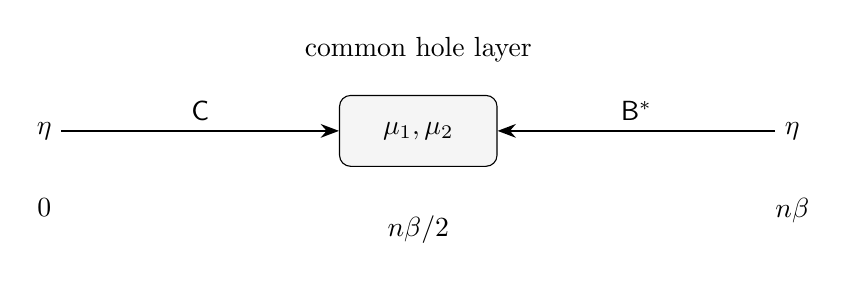
\begin{tikzpicture}[>=Stealth,scale=0.95]
 \node (left) at (0,0) {$\eta$};
 \node[draw,rounded corners,fill=gray!8,minimum height=9mm,minimum width=20mm]
       (mid) at (5,0) {$\mu_1,\mu_2$};
 \node (right) at (10,0) {$\eta$};
 \draw[->,thick] (left) -- node[above] {$\mathsf C$} (mid);
 \draw[->,thick] (right) -- node[above] {$\mathsf B^*$} (mid);
 \node[below=5mm of left] {$0$};
 \node[above=3mm of mid] {common hole layer};
 \node[below=5mm of mid] {$n\beta/2$};
 \node[below=5mm of right] {$n\beta$};
\end{tikzpicture}
\caption{A diagonal return is an inner product on the midpoint layer.
Both masses use the same exposure, with fresh transitions in each
traversal. Coupling either mass to an independent full ideal path gives
an expected \(\ell^1\) error; diffusion bounds the other mass in
\(\ell^\infty\). The positions are elapsed times, not lattice sites.}
\label{fig:midpoint}
\end{figure}

Let \(G\) be the good-exposure event for \(z,R\). Each half has
elapsed length \(n\beta/2\ge\beta/2\), so
Proposition~\ref{prop:diffusion}, including its adjoint statement,
gives \(\|\mu_1\|_\infty+\|\mu_2\|_\infty\le C\beta^{-3/2}\)
on \(G\). The ideal halves obey this bound without a good-exposure
condition: each slot probability is bounded by its full site
probability in \eqref{eq:ideal-site-bounds}. A half need not contain
a seam for this upper bound. The elementary pairing inequality gives
\begin{align}
 &\left|\mathbb E_P[(W_R)_{ii}]-(\widehat W_R)_{ii}\right|\notag\\
 &\quad\le C\beta^{-3/2}\mathbb E_P
    \left[\|\mu_1-\widehat\mu_1\|_1+
          \|\mu_2-\widehat\mu_2\|_1\right]
       +\mathbb P_P(G^c).\label{eq:midpoint-reduction}
\end{align}
Indeed on \(G\) subtract the two inner products by changing their
first and second arguments successively; on \(G^c\) both diagonal
entries lie in \([0,1]\). No independence of the two halves is used.
Since \(\mathbb P_P(G^c)=o_K(\beta^{-3/2})\), it remains to prove
\begin{equation}\label{eq:coupling-l1}
 \mathbb E_P\|\mu_j-\widehat\mu_j\|_1=o_K(1),\qquad j=1,2.
\end{equation}

\medskip\noindent
\emph{Coupling conditional on the exposure.}
Both masses are generated from \(i\) along a deterministic schedule
of full or partial traversals. For \(j=2\), reverse and transpose the
suffix factors. We give the coupling for either schedule. Sample the
entire actual picture with law \(\mathbb P_P\) and expose
\(\mathcal B_P\). Independently of that entire picture, sample a
full unkilled ideal path on the infinite slot lattice, with fresh
clocks and seam permutations on each traversal. Its bounded jump rate
\(\lambda_J\) ensures that it is well defined. Conditional on the
exposure, use the same fresh clock on each slot edge whenever its
endpoints are holes in the cube. At a prescribed exposed jump, perform
the corresponding hole transport. At a seam, share the uniform site
permutation if the site has no exposed slots; otherwise use an
appropriate fresh uniform completion on its remaining slots. These
rules give exactly the hole kernel conditional on the exposure. They
also apply to reverse pieces: heat generators are symmetric, transports
are inverted, and inverse uniform bijections are uniform. Repeated
traversals share the exposure but use independent fresh transitions.

Kill both paths outside \(\Lambda^\circ\) or
\(\mathfrak B_R(z)\). Until they separate these killings agree.
There are no interaction bonds from \(\Lambda^\circ\) to the
exterior of \(\Lambda\), by the choice of boundary thickness.
A discrepancy before killing therefore requires an exposed slot at a
site whose bar-coordinate is within distance \(2B_*\) of the full
ideal path, at some traversed time. Include both sides of jumps and
instantaneous operations in this event. This covers a missing clock
edge, a forced transport affecting the common path, and a seam
completion different from a full site permutation.

\medskip\noindent
\emph{Averaged encounter bound.}
We bound the probability of this encounter unconditionally. Partition
the schedule into \(O_K(\beta)\) deterministic intervals of elapsed
length at most one, each within a single directed traversal piece;
assign endpoint operations once. Take
\(h_\beta=\lceil\log\beta\rceil\). In one such interval let
\(w\) be the bar-coordinate of the full ideal path at its initial
time. Since each jump changes bar-coordinate by at most \(B_*\),
the probability of displacement greater than \(B_*h_\beta\) during
the interval is at most
\begin{equation}\label{eq:ideal-short-tail}
 \frac{C^{h_\beta}}{h_\beta!}.
\end{equation}
For a deterministic \(w\), Corollary~\ref{cor:singleton-bound},
applied with pin set \(P\) and summed over slots, gives
\begin{equation}\label{eq:encounter-initial}
 \mathbb P_P\!\left(
  \text{an exposed slot lies over }
  \mathfrak B_{4B_*(h_\beta+1)}(w)
  \text{ at the initial slice}\right)
 \le C(h_\beta+1)^3\beta^{-3/2}.
\end{equation}
At a seam the set of sites occupied by exposed slots is the same on
both sides, so this estimate covers either endpoint convention.

If this initial event is absent but an exposed strand subsequently
visits \(\mathfrak B_{B_*(h_\beta+2)}(w)\) in the interval, trace
that strand back toward the initial slice. The distance between the
two regions forces at least \(h_\beta\) inter-site steps. Count the
first \(h_\beta\) steps from a visit. Their actual marks are distinct:
this interval lies in one traversal, and for large \(\beta\) its
length is less than \(\beta\), so unwrapped physical time is monotone
and injective modulo \(\beta\). There are at most
\(C(h_\beta+1)^3\) starting sites in the smaller region and a bounded
number of next-site and slot-edge choices per step. By the factorial
measure domination of Lemma~\ref{lem:factorial}, the probability of
such a list is at most
\begin{equation}\label{eq:encounter-entrance}
 C(h_\beta+1)^3 C^{h_\beta}
  \int_{0<s_1<\cdots<s_{h_\beta}<1}ds_1\cdots ds_{h_\beta}
 =C(h_\beta+1)^3\frac{C^{h_\beta}}{h_\beta!}.
\end{equation}
Discarding slot compatibility only enlarges the count. A seam can
change a slot index but no site, so it merely contributes a bounded
slot choice; unwrapping preserves the simplex volume. Reversing a
traversal reverses the order of the times and gives the same bound.
Thus \eqref{eq:encounter-entrance} uses factorial domination under the
full picture law, without conditioning that domination on the exposure.

The random coordinate \(w\) depends only on the independent full ideal
path. The bounds \eqref{eq:encounter-initial} and
\eqref{eq:encounter-entrance}, uniform for deterministic \(w\) and
deterministic initial times, therefore apply to this random \(w\).
A union bound over the intervals bounds the encounter probability by
\begin{equation}\label{eq:encounter-probability}
 C_K\beta(h_\beta+1)^3
       \left(\beta^{-3/2}+\frac{C^{h_\beta}}{h_\beta!}\right)
 =o_K(1).
\end{equation}
The first term is \(O_K(\beta^{-1/2}(\log\beta)^3)\); the factorial
term decays faster than every fixed inverse power of \(\beta\).
Actual marks may reappear in later traversals, but the count used
distinctness only within one interval. The union bound needs no
independence across these intervals.

Add a death state for killing. Conditional on each exposure, the
\(\ell^1\) distance between the two live output masses is at most
twice the failure probability of this coupling. Average over the
picture and use \eqref{eq:encounter-probability}. This proves
\eqref{eq:coupling-l1} for both schedules and, by
\eqref{eq:midpoint-reduction}, proves \eqref{eq:finite-word}.
\end{proof}

\subsection{Uniform return and down-spin bounds}

\begin{theorem}[One-slot bounds with the sharp coefficient]
\label{thm:return-bounds}
There is a constant \(C<\infty\), independent of \(K\), with the
following property. For every integer \(K\ge1\) there are
\(\beta_K<\infty\) and a nonnegative function
\(\epsilon_K(\beta)\to0\) as \(\beta\to\infty\), such that for
\(\beta\ge\beta_K\), every finite cube, every allowed pin set
\(E\), and every deterministic slot-time point \(i\),
\begin{equation}\label{eq:down-upper}
 d_E(i)\le\beta^{-3/2}
 \left(\frac\kappa\ell\sum_{n=1}^{2K-1}n^{-3/2}
                  +CK^{-1/2}+\epsilon_K(\beta)\right).
\end{equation}
If the site \(x\) of \(i\) additionally satisfies
\begin{equation}\label{eq:pin-free-ball}
 \mathfrak B_{R_K}(\bar x)\subseteq\Lambda^\circ,
 \qquad E\text{ has no pin over }\mathfrak B_{R_K}(\bar x),
\end{equation}
then
\begin{equation}\label{eq:down-lower}
 d_E(i)\ge\beta^{-3/2}
 \left(\frac\kappa\ell\sum_{n=1}^{K}n^{-3/2}
                                      -\epsilon_K(\beta)\right).
\end{equation}
For \(i\notin E\), the same two bounds hold for \(r(E,\{i\})\),
with the same choice of error function. The threshold and error
function are independent of the cube, cut, slot, and number, locations,
and times of all finite extra pins. Only the fixed model and geometric
choices, and \(K\), may affect them.
\end{theorem}

\begin{proof}
Suppose first that \(i\notin E\), and take the exposure law
\(\mathbb P_P\), \(P=E\cup\{i\}\). Lemma~\ref{lem:return-expansion}
and Proposition~\ref{prop:long-tail} give
\[
 r(E,\{i\})\le
 \sum_{n=1}^{2K-1}\mathbb E_P\langle\eta,Q^n\eta\rangle
 +\beta^{-3/2}\bigl(CK^{-1/2}+o_K(1)\bigr).
\]
Expand \(Q^n\) as the equally weighted average of the \(2^n\)
direction words. Replacing each word by its localized version costs
at most \(C_Ke^{-c\beta}\) in expected diagonal mass, by
Lemma~\ref{lem:localization}. Proposition~\ref{prop:finite-word} and
Lemma~\ref{lem:ideal-kernel} then imply
\[
 r(E,\{i\})\le\beta^{-3/2}
 \left(\frac\kappa\ell\sum_{n=1}^{2K-1}n^{-3/2}
                   +CK^{-1/2}+o_K(1)\right).
\]
There are only finitely many words at fixed \(K\), so all comparison
errors enter \(o_K(1)\). They do not alter the constant multiplying
\(K^{-1/2}\).

For the lower bound assume \eqref{eq:pin-free-ball}. At fixed exposure,
run the forward fresh walk with boundary and ball killing, and continue
it after visits to \(i\). Let \(A_n\) be the event that it is alive
and at \(i\) at elapsed time \(n\beta\). Before any such visit it
has stayed in the ball and hence avoided \(E\). Thus
\(q_i\ge\Pr(\bigcup_{n=1}^K A_n\mid\text{exposure})\).
The fresh transitions on successive turns give
\[
 \Pr(A_n\mid\text{exposure})=(U_{+,R}^n)_{ii},\qquad
 \Pr(A_j\cap A_n\mid\text{exposure})
     =(U_{+,R}^j)_{ii}(U_{+,R}^{n-j})_{ii}\quad(j<n).
\]
The Bonferroni lower bound therefore reads
\begin{equation}\label{eq:bonferroni}
 q_i\ge\sum_{n=1}^K(U_{+,R}^n)_{ii}
 -\sum_{1\le j<n\le K}
       (U_{+,R}^j)_{ii}(U_{+,R}^{n-j})_{ii}.
\end{equation}
On good exposures each product is \(O(\beta^{-3})\) by
Proposition~\ref{prop:diffusion}; on the complement each is at most
one, and that complement has probability \(o_K(\beta^{-3/2})\).
The expected pair sum is consequently \(o_K(\beta^{-3/2})\).
For the first sum apply Proposition~\ref{prop:finite-word} to the
all-forward word and use the interior comparison
\eqref{eq:ideal-killed-interior}. Averaging \eqref{eq:bonferroni}
gives
\[
 r(E,\{i\})\ge\beta^{-3/2}
 \left(\frac\kappa\ell\sum_{n=1}^{K}n^{-3/2}-o_K(1)\right).
\]

Finally, Proposition~\ref{prop:pin-identities} and
Corollary~\ref{cor:singleton-bound} give, uniformly,
\[
 d_E(i)=\frac{r(E,\{i\})}{1+r(E,\{i\})},\qquad
 0\le r(E,\{i\})-d_E(i)\le C\beta^{-3}.
\]
This changes only the normalized \(o_K(1)\) errors. Choose a common
threshold \(\beta_K\) and a nonnegative error function tending to
zero that dominates all these uniform error magnitudes. This proves
both estimates for \(r\) and \(d\). If \(i\in E\), then
\(d_E(i)=0\), so the upper bound still holds; the lower-bound
hypotheses already exclude this case.
\end{proof}

\section{From pinned returns to spontaneous magnetization}
\label{sec:pressure}

The return estimates hold for every deterministic choice of extra pins.
A positive magnetic field is an exact mixture of such choices. We use
this fact to bound finite-volume pressure increments, then take the
thermodynamic limit before differentiating at zero field.

\subsection{Pressure and the cost of boundary pins}

Write $V=|\Lambda_N|$ and
\[
 p_N(h)=\frac1{\beta V}\log Z_{\Lambda_N}(h).
\]
The limit $p_\beta(h)=\lim_{N\to\infty}p_N(h)$ exists for every
$\beta>0$ and $h\in\R$. Here is the finite-range argument. Tile a large
cube, apart from a remainder, by cubes of a fixed side $l$ and delete
all interactions between tiles. There are $O(V/l)$ deleted bonds,
each with uniformly bounded operator norm; the remainder has $o(V)$
sites as $N\to\infty$ with $l$ fixed and may be left as singletons.
If two Hamiltonians differ by an operator of norm at most $a$, their
logarithmic partition functions differ by at most $\beta a$, by
ordered-eigenvalue comparison. Consequently the limiting upper and
lower pressures both lie within $C/l$ of the pressure per site of a
single tile. Letting $l\to\infty$ proves existence. Since
$[H^J_{S,N},M_{S,N}]=0$ and $\norm{M_{S,N}}\le SV$, each $p_N$ is
convex and $S$-Lipschitz in $h$. These properties pass to $p_\beta$,
so its right derivative at zero exists.

Let $Z^+_\Lambda(h)$ be the loop expression in
Proposition~\ref{prop:loop-representation} with all cycles meeting
$D_0$ constrained to have color $+1$, and put
$p_N^+(h)=(\beta V)^{-1}\log Z^+_{\Lambda_N}(h)$.

\begin{proposition}[Boundary pressure equivalence]
\label{prop:pressure-equivalence}
For every fixed $\beta>0$ and $h\ge0$,
\begin{equation}
 \lim_{N\to\infty}p_N^+(h)=p_\beta(h).
 \label{eq:boundary-pressure}
\end{equation}
\end{proposition}

\begin{proof}
Factor $e^{\beta hSV}$ from the unrestricted color sum. Its picture
weight, relative to the base law, becomes
\[
 W_h=\prod_C(1+e^{-\beta h a_C}).
\]
Given the picture, the colors of different cycles are independent and
the probability that a cycle is up is at least $1/2$. If $b_\partial$
counts the cycles meeting $D_0$, the corresponding normalized picture
expectation therefore satisfies
\begin{equation}
 1\ge \frac{Z^+_\Lambda(h)}{Z_\Lambda(h)}
 \ge \mathbb E_h[2^{-b_\partial}]
 \ge \exp\{-\log(2)\,\mathbb E_h b_\partial\}.
 \label{eq:surface-cost}
\end{equation}
A cycle visiting the boundary either contains a time-zero boundary
slot or arrives there at a mark incident to the boundary. Thus
\[
 b_\partial\le \ell|\partial\Lambda|+2N_\partial,
\]
where $N_\partial$ is the number of such marks. Insertion of a mark
changes at most two cycle factors in $W_h$, each between one and two,
so it increases $W_h$ by at most a factor of four. The Poisson insertion
argument of Lemma~\ref{lem:factorial} gives
$\mathbb E_hN_\partial\le C\beta|\partial\Lambda|$.
Taking logarithms in \eqref{eq:surface-cost} yields
\[
 0\le p_N(h)-p_N^+(h)
 \le C(1+\beta)\frac{|\partial\Lambda|}{\beta|\Lambda|}.
\]
For fixed $\beta$, the right side tends to zero.
\end{proof}

\subsection{A magnetic field as random extra pins}

The mixture in the next lemma is useful because its conditional laws
are precisely the deterministic pin laws already studied. Its mixing
measure need not be a product measure.

\begin{lemma}[Extra-pin mixture]
\label{lem:pin-mixture}
For $h\ge0$, the colored-picture law defining $Z^+_\Lambda(h)$ is
a mixture of the zero-field pinned laws with pin sets $E=D_0\cup F$,
where $F$ consists of time-zero slots. Under the mixing law,
\begin{equation}
 \Pr(i\in F)\le b(h):=1-e^{-\beta h}
 \qquad\text{for every time-zero slot }i.
 \label{eq:pin-marginal}
\end{equation}
Moreover,
\begin{equation}
 S-(p_N^+)'(h)
   =\frac1V\sum_{i\in V_\Lambda}\mathbb E_F[d_{D_0\cup F}(i)].
 \label{eq:field-deficit}
\end{equation}
\end{lemma}

\begin{proof}
For a colored picture let $D_{\rm down}$ count its down slots at time
zero. Then $M=SV-D_{\rm down}$. Start with independent selection of
all time-zero slots with probability $b(h)$. The probability that
only up slots are selected is
$(1-b(h))^{D_{\rm down}}=e^{-\beta hD_{\rm down}}$.
Consequently the joint weight obtained by multiplying the zero-field
colored-picture weight by the independent selection weight and by
$\ind{F\text{ contains only up slots}}$ has exactly the desired
field-tilted colored-picture marginal, after normalization.
Conditioning instead on $F$ leaves unit weight for each coloring
satisfying the pins $D_0\cup F$. Summing these colorings gives the
picture factor $2^{n_{D_0\cup F}}$, as required.

Conditional on the picture and its colors in this joint law, down
slots are never selected, while up slots are selected independently
with probability $b(h)$. This proves \eqref{eq:pin-marginal}.
Finally, differentiation of the finite-volume field tilt gives
$(p_N^+)'(h)=V^{-1}\mathbb E M$; conditioning on $F$ gives
\eqref{eq:field-deficit}.
\end{proof}

\subsection{The order of limits}

Recall the ideal heat-kernel constant and define its finite sums by
\begin{equation}
 \kappa=\frac1{(4\pi)^{3/2}\sqrt{\det D_{S,J}}},
 \qquad c_j=\kappa\sum_{n=1}^j n^{-3/2}.
 \label{eq:partial-bloch}
\end{equation}
Fix an integer $K\ge1$ and use the radius
$R=R_K=\lceil a(K+1)\beta\rceil$ from \eqref{eq:scales}.
The upper down-probability bound of Theorem~\ref{thm:return-bounds}
and \eqref{eq:field-deficit} imply
\begin{equation}
 S-(p_N^+)'(h)
 \le\beta^{-3/2}
       \bigl(c_{2K-1}+CK^{-1/2}+\epsilon_K(\beta)\bigr),
 \label{eq:pressure-upper}
\end{equation}
where $\epsilon_K(\beta)\ge0$ tends to zero as $\beta\to\infty$ for
fixed $K$, uniformly in $N$ and $h\ge0$. The leading constant $C$
is independent of $K$. There are $\ell V$ slots in the sum, so the
factor $1/\ell$ in each ideal slot-return probability has canceled.

For a lower bound, let $\rho_N$ be the fraction of sites $x\in\Lambda_N$
for which $\mathfrak B_R(\bar x)\subseteq\Lambda_N^\circ$. Since the
coset representatives and $A$ are fixed, all sites in this ball lie
within a bounded physical distance of $x$ when $R$ is fixed. Hence
$\rho_N\to1$ as $N\to\infty$, with $\beta,K$ fixed.
There are at most
\[
 v_R=\ell|\mathfrak C|(2R+1)^3
\]
time-zero slots above the ball. The union bound and
\eqref{eq:pin-marginal} show that it contains no extra pin with
probability at least $[1-v_Rb(h)]_+$, where $[u]_+=\max\{u,0\}$.
On this event Theorem~\ref{thm:return-bounds} supplies its lower bound.
Enlarging $\epsilon_K$ to cover both errors gives
\begin{equation}
 S-(p_N^+)'(h)
 \ge\rho_N[1-v_Rb(h)]_+\,
       \beta^{-3/2}\bigl(c_K-\epsilon_K(\beta)\bigr).
 \label{eq:pressure-lower}
\end{equation}
Here and below $\beta$ is sufficiently large, depending on $K$, that
$c_K-\epsilon_K(\beta)\ge0$.

\begin{proof}[Proof of Theorem~\ref{thm:main}]
Integrate \eqref{eq:pressure-upper} and \eqref{eq:pressure-lower}
from $0$ to $h>0$, and divide by $h$. This bounds
\[
 S-\frac{p_N^+(h)-p_N^+(0)}{h}.
\]
First send $N\to\infty$, using Proposition~\ref{prop:pressure-equivalence}
at both endpoints and $\rho_N\to1$. Then send $h\downarrow0$.
For these fixed $\beta,K$, continuity of $b$ at zero gives
\[
 \lim_{h\downarrow0}\frac1h\int_0^h[1-v_Rb(u)]_+\,du=1.
\]
By the definition of the right derivative,
\begin{equation}
 c_K-\epsilon_K(\beta)
 \le\beta^{3/2}\bigl(S-m_{S,J}(\beta)\bigr)
 \le c_{2K-1}+CK^{-1/2}+\epsilon_K(\beta).
 \label{eq:final-squeeze}
\end{equation}
Thus the thermodynamic limit and the zero-field derivative have been
handled through pressure increments. Now let $\beta\to\infty$ with
$K$ fixed and then $K\to\infty$. Both sides of
\eqref{eq:final-squeeze} converge to $\kappa\zeta(3/2)$, proving
the stated law.
\end{proof}

\begin{thebibliography}{99}

\bibitem{BjornbergRyan2026}
J.~E.~Bj\"ornberg and K.~Ryan.
Exponential decay in \(\mathcal O(n)\)-invariant quantum spin systems.
\emph{Annales Henri Poincar\'e} (2026), published online March~25, 2026.
\href{https://doi.org/10.1007/s00023-026-01690-3}{doi:10.1007/s00023-026-01690-3}.

\bibitem{Bloch1930}
F.~Bloch.
Zur Theorie des Ferromagnetismus.
\emph{Zeitschrift f\"ur Physik} \textbf{61} (1930), 206--219.
\href{https://doi.org/10.1007/BF01339661}{doi:10.1007/BF01339661}.

\bibitem{BBL2009}
J.~Borcea, P.~Br\"and\'en, and T.~M.~Liggett.
Negative dependence and the geometry of polynomials.
\emph{Journal of the American Mathematical Society}
\textbf{22} (2009), 521--567.
\href{https://doi.org/10.1090/S0894-0347-08-00618-8}{doi:10.1090/S0894-0347-08-00618-8}.

\bibitem{ConlonSolovej1991}
J.~G.~Conlon and J.~P.~Solovej.
Upper bound on the free energy of the spin~\(1/2\) Heisenberg ferromagnet.
\emph{Letters in Mathematical Physics} \textbf{23} (1991), 223--231.
\href{https://doi.org/10.1007/BF01885500}{doi:10.1007/BF01885500}.

\bibitem{CGS2015}
M.~Correggi, A.~Giuliani, and R.~Seiringer.
Validity of the spin-wave approximation for the free energy of the
Heisenberg ferromagnet.
\emph{Communications in Mathematical Physics} \textbf{339} (2015), 279--307.
\href{https://doi.org/10.1007/s00220-015-2402-0}{doi:10.1007/s00220-015-2402-0}.

\bibitem{Dyson1956a}
F.~J.~Dyson.
General theory of spin-wave interactions.
\emph{Physical Review} \textbf{102} (1956), 1217--1230.
\href{https://doi.org/10.1103/PhysRev.102.1217}{doi:10.1103/PhysRev.102.1217}.

\bibitem{Dyson1956b}
F.~J.~Dyson.
Thermodynamic behavior of an ideal ferromagnet.
\emph{Physical Review} \textbf{102} (1956), 1230--1244.
\href{https://doi.org/10.1103/PhysRev.102.1230}{doi:10.1103/PhysRev.102.1230}.

\bibitem{DLS1978}
F.~J.~Dyson, E.~H.~Lieb, and B.~Simon.
Phase transitions in quantum spin systems with isotropic and nonisotropic
interactions.
\emph{Journal of Statistical Physics} \textbf{18} (1978), 335--383.
\href{https://doi.org/10.1007/BF01106729}{doi:10.1007/BF01106729}.

\bibitem{FSS1976}
J.~Fr\"ohlich, B.~Simon, and T.~Spencer.
Infrared bounds, phase transitions and continuous symmetry breaking.
\emph{Communications in Mathematical Physics} \textbf{50} (1976), 79--95.
\href{https://doi.org/10.1007/BF01608557}{doi:10.1007/BF01608557}.

\bibitem{HolsteinPrimakoff1940}
T.~Holstein and H.~Primakoff.
Field dependence of the intrinsic domain magnetization of a ferromagnet.
\emph{Physical Review} \textbf{58} (1940), 1098--1113.
\href{https://doi.org/10.1103/PhysRev.58.1098}{doi:10.1103/PhysRev.58.1098}.

\bibitem{Lieb1999}
E.~H.~Lieb.
Long range order for the quantum Heisenberg model.
\emph{Open Problems in Mathematical Physics}, contribution dated
January~27, 1999, Problem~A.
\href{https://web.math.princeton.edu/~aizenman/OpenProblems_MathPhys/9901.HeisenbergFerr.html}{Author's problem statement}.

\bibitem{MerminWagner1966}
N.~D.~Mermin and H.~Wagner.
Absence of ferromagnetism or antiferromagnetism in one- or two-dimensional
isotropic Heisenberg models.
\emph{Physical Review Letters} \textbf{17} (1966), 1133--1136;
erratum, \textbf{17} (1966), 1307.
\href{https://doi.org/10.1103/PhysRevLett.17.1133}{doi:10.1103/PhysRevLett.17.1133}.

\bibitem{Nachtergaele1994}
B.~Nachtergaele.
Quasi-state decompositions for quantum spin systems.
In B.~Grigelionis et al. (eds.),
\emph{Probability Theory and Mathematical Statistics},
Proceedings of the Sixth Vilnius Conference,
VSP/TEV, Utrecht--Tokyo--Vilnius, 1994, pp.~565--590.
\href{https://arxiv.org/abs/cond-mat/9312012}{arXiv:cond-mat/9312012}.

\bibitem{Nash1958}
J.~Nash.
Continuity of solutions of parabolic and elliptic equations.
\emph{American Journal of Mathematics} \textbf{80} (1958), 931--954.
\href{https://doi.org/10.2307/2372841}{doi:10.2307/2372841}.

\bibitem{Ordering}
OpenAI.
\emph{Spontaneous magnetization in the quantum Heisenberg ferromagnet}.
OpenAI Math Release preprint
\href{https://github.com/openai/math/blob/main/preprints/Spontaneous-magnetization-in-the-quantum-Heisenberg-ferromagnet-September-24-2026/paper.pdf}{OAI:Spontaneous-magnetization-in-the-quantum-Heisenberg-ferromagnet-September-24-2026},
2026.

\bibitem{Seiringer2025}
R.~Seiringer.
The Heisenberg ferromagnet: a dilute Bose gas in disguise.
In \emph{Mini-Workshop: New Directions in Correlated Quantum Systems},
\emph{Oberwolfach Reports} \textbf{22} (2025), 357--358.
\href{https://doi.org/10.4171/OWR/2025/7}{doi:10.4171/OWR/2025/7}.

\bibitem{Toth1993}
B.~T\'oth.
Improved lower bound on the thermodynamic pressure of the spin~\(1/2\)
Heisenberg ferromagnet.
\emph{Letters in Mathematical Physics} \textbf{28} (1993), 75--84.
\href{https://doi.org/10.1007/BF00739568}{doi:10.1007/BF00739568}.

\end{thebibliography}

\end{document}
